%%
%% This is file `thesis-test.tex',
%% generated with the docstrip utility.
%%
%% The original source files were:
%%
%% nuthesis.dtx  (with options: `thesis-test')
%% 

\documentclass[ms]{nuthesis}
%% Needed to typset the math in this sample
\usepackage{amsmath}
\usepackage{amsfonts}
%% Let's use a different font
\usepackage[sc,osf]{mathpazo}

%% prevents placing floats before a section
\usepackage[section]{placeins}

%% Makes things look better
\usepackage{microtype}

%% Makes things look better
\usepackage{booktabs}

%% Gives us extra list environments
\usepackage{paralist}

%% Be able to include graphicsx
\usepackage{graphicx}

%% Be able to use subfigure
\usepackage{caption}
\usepackage{subcaption}

% Make caption have a universal width
%\usepackage[width=.75\textwidth]{caption}

%% Make tables with set width
\usepackage{tabularx}

%% make tables closer
\usepackage{float}

%% I like darker colors
\usepackage{color}
\definecolor{dark-red}{rgb}{0.6,0,0}
\definecolor{dark-green}{rgb}{0,0.6,0}
\definecolor{dark-blue}{rgb}{0,0,0.6}

%% If you use hyperref, you need to load memhfixc *after* it.
%% See the memoir docs for details.
\usepackage[%
pdfauthor={James D. Duin},
pdftitle={Hierarchical Active Learning Bioinformatics Application},
pdfsubject={BioDataset},
pdfkeywords={semi-supervised learning, active learning, hierarchical labeling, cost analysis},
linkcolor=dark-blue,
pagecolor=dark-green,
citecolor=dark-blue,
urlcolor=dark-red,
%colorlinks=true,
backref,
plainpages=false,% This helps to fix the issue with hyperref with page numbering
pdfpagelabels% This helps to fix the issue with hyperref with page numbering
]{hyperref}

%% Needed by memoir to fix things with hyperref
\usepackage{memhfixc}
\begin{document}
%% Start formating the first few special pages
%% frontmatter is needed to set the page numbering correctly
\frontmatter

\title{Hierarchical Active Learning Bioinformatics Application}
\author{James D. Duin}
\adviser{Professor Stephen Scott}
\adviserAbstract{Stephen Scott}
\major{Computer Science}
\degreemonth{March}
\degreeyear{2017}
%%
%% For most people the defaults will be correct, so they are commented
%% out. To manually set these, just uncomment and make the needed
%% changes.
%% \college{Your college}
%% \city{Your City}
%%
%% For most people the following can be changed with a class
%% option. To manually set these, just uncomment the following and
%% make the needed changes.
%% \doctype{Thesis or Dissertation}
%% \degree{Your degree}
%% \degreeabbreviation{Your degree abbr.}
%%
%% Now that we know everything we need, we can generate the title page
%% itself.
%%
\maketitle
%% You have a maximum of 350, which includes your title, name, etc.
\begin{abstract}
  \par This study investigates an application of the Support Vector Machine
   and Logistic Regression machine learning algorithms to a protein dataset labeled
   according to a proteins location of origin in a cell. The dataset is labeled
   according to a
    hierarchical scheme, at the root level the protein is from the mitochondria
    or not, then the hierarchy breaks down further into specific target
    compartments at the leaf nodes. Our investigation shows that Leveraging separate
    fine-grained classifiers for each of the target compartments produces a higher
    performing classifier at the highest level in the hierarchy according
    to the Precision-Recall curves area under the curve. Furthermore, new approach in the
     Active Learning setting termed \textit{active over-labeling} is applied to this dataset.
    The approach solicits labels at a finer level of granularity than the target concept.
    We show that purchasing fine-grained labels in each round of active learning produces a
      higher performing classifier than purchasing coarse labels, and in both cases purchasing
      labels actively by selecting only the most uncertain labels outperforms purchasing labels
      passively, i.e. at random. The fine-grained labels also incur a higher cost than coarse-grained
      labels for this dataset, so multiple cost ratios ran and an optimal Fixed Fine
      ratio purchasing strategy is determined for each fine cost.
\end{abstract}

%% Optional
%\begin{copyrightpage}
%This file may be distributed and/or modified under the conditions of
%the \LaTeX{} Project Public License, either version 1.3c of this license
%or (at your option) any later version.  The latest version of this
%license is in:
%\begin{center}
%   \url{http://www.latex-project.org/lppl.txt}
%\end{center}
%and version 1.3c or later is part of all distributions of \LaTeX version
%2006/05/20 or later.
%\end{copyrightpage}

%% Optional
\begin{dedication}
  This thesis is dedicated to my parents Paul and Vicki Duin and fianc\'{e}e Anna Spady.
\end{dedication}

%% Optional
\begin{acknowledgments}
  I would like to thank my advisor Dr. Stephen Scott for guidance in selecting this
  research topic, Yugi Mo for his work in developing the HAL methodology, and Dr.
  Douglas Downey for his work on this topic. I would like to thank Juan Cui, Jiang Shu,
  Kevin Chiang for assistance accessing and understanding the protein dataset that is
  the subject of the paper.
\end{acknowledgments}

%% Optional
%\begin{grantinfo}
%  I'm not funded by any grants.
%\end{grantinfo}
%%% The ToC is required
%%% Uncomment these if need be

%% The ToC is required
\tableofcontents
%% Uncomment these if need be
%\listoffigures
%\listoftables

%%   mainmatter is needed after the ToC, (LoF, and LoT) to set the
%%   page numbering correctly for the main body
\mainmatter

%% Thesis goes here
\chapter{Introduction}



\section{Machine Learning}
\par Machine learning (ML) algorithms are defined as computer programs that learn from experience E
with respect to some class of tasks T and performance measure P, if their performance at
tasks in T, as measured by P, improves with experience E \cite{mitchell}. In the context of this paper,
the machine learning algorithms that are used include Support Vector Machines (SVM), and Logistic Regression (Logit).
 This work uses implementations by the sci-kit learn python library \cite{scikit-learn} for both algorithms. Our
 experiment requires a binary classification task, each algorithm takes a protein instance with a list of 449 features
 as an input and then outputs a 0 or 1 whether or not the protein belongs to a class. A separate classifier is trained
 for each class in the protein dataset. Both Logit and SVM classifiers have a decision function method that outputs
 the predicted confidence score for a given sample, which is the signed distance of that sample to the learned
 hyperplane.
 \par Logit is a linear model for classification. The classifier function is shown in \textit{eqn. \ref{eq:logit}}.
 Where x is the vector of features, theta is vector of learned parameters, the function $g(z)$ is the sigmoid
 function \cite{Coursera}.
\FloatBarrier
\begin{equation}
\label{eq:logit}
\begin{aligned}
h_{\theta}(x) = g(\theta \cdot x) \\
g(z) = \frac{1}{1+e^{-z}}
\end{aligned}
\end{equation}
\FloatBarrier
The theta parameters are solved for in order to minimize the sum of square errors (L2-norm)
in the training set, and also to regularize the theta parameters to prevent them from getting to large
and overfitting the dataset \cite{scikit-learn}. A cost function is used to solve for theta, this
function is shown in \textit{eqn \ref{eq:costlogit}}. The $C$ parameter is the inverse of the regularization
strength, a larger value means a stronger regularization \cite{scikit-learn}.
\FloatBarrier
\begin{equation}
\label{eq:costlogit}
\begin{aligned}
min_{\theta,c}\frac{1}{2}\theta^{T}\theta + C\sum_{n}^{i=1}log(exp(-y_i(X_{i}^{T}\theta+c))+1)
\end{aligned}
\end{equation}
\FloatBarrier
\par A SVM constructs a hyper-plane or set of hyper-planes in a high or infinite dimensional space, which
is used to output a classification for a given instance. The goal is to learn a hyper-plane that has
the largest distance between training data points of separate classes, this is called functional margin
\cite{scikit-learn}. In general the larger the functional margin the lower the generalized error of the
classifier. SVMs are a maximum functional margin method that allow the model to be written as a sum of the
influence of a subset of the training instances \cite{ethem}. This output is given by kernel functions
that are measures of similarity between data instances. The SVM implementation used solves the
\textit{eqn. \ref{eq:svmfcn}}, where $e$ is a vector of all ones, $C$ is the penalty parameter of the
error term.
\FloatBarrier
\begin{equation}
\label{eq:svmfcn}
\begin{aligned}
min_{\alpha} \frac{1}{2} \alpha^{T} Q\alpha - e^T\alpha, \
subject\  to\ y^T \alpha = 0 \ where\ 0\leq\alpha_i\leq C,i=1,...,n
\end{aligned}
\end{equation}
\FloatBarrier
The $Q$ function is defined in \textit{eqn. \ref{eq:kernelfcn}}, where $K$ is the kernel function.
\FloatBarrier
\begin{equation}
\label{eq:kernelfcn}
\begin{aligned}
Q_{ij}\equiv y_i y_j K(x_i,x_j), \ where \ K(x_i,x_j)=\phi (x_i)^T \phi(x_j)
\end{aligned}
\end{equation}
\FloatBarrier

The $C$ parameter trades off misclassification of training examples against simplicity of the
decision surface \cite{scikit-learn}. A low $C$ makes the decision surface smooth, while a high $C$ aims at
classifying all the training examples correctly by allowing the model to select more samples as support
vectors \cite{scikit-learn}. The gamma ($\gamma$) parameter defines the significance a single training example
 can have, with low values corresponding to a single instance having a large significance to the
 learned hyperplane \cite{scikit-learn}. The gamma parameter can be seen as the inverse of the radius of
 influence of samples selected by the model as support vectors.

In this work the following kernel functions were tested \cite{scikit-learn}:
\begin{itemize}
  \item linear: $\left \langle x,x^{'} \right \rangle$
  \item polynomial: $(\gamma \left \langle x,x^{'} \right \rangle + r)^{d}$. $d$ is the degree
  of the polynomial, and $r$ is a coefficient passed to the solver, default is $0$.
  \item radial basis function (rbf): $(-\gamma |x-x^{'}|^{2})$. $\gamma$ is the kernel coefficient.
  \item sigmoid: $sigmoid(tanh(\gamma \left \langle x,x^{'} \right \rangle + r))$
  $r$ is a coefficient passed to the solver, default is $0$.
\end{itemize}


\section{Evaluating Classifier Performance}
\par The classifier performance is primarily evaluated using Precision-Recall (PR) and Receiver Operator
Characteristic (ROC) curves, although accuracy, precision, recall, confusion matrix and  F-measure
are also calculated. Accuracy is the total number of correctly classified instances in the test set
divided by the total number of instances in the test set. The confusion matrix outputs a 2 by 2 matrix
for the binary classification task. Each cell ($C_{row,col}$) in the matrix corresponds to one of the
following metrics:
\begin{itemize}
  \item True-Negatives ($T_n$): location $C_{0,0}$, correctly classified negative instances.
  \item False-Negatives ($F_n$): location $C_{0,1}$, incorrectly classified negative instances.
  \item False-Positives ($F_p$): location $C_{1,0}$, incorrectly classified positive instances.
  \item True-Positives ($T_p$): location $C_{1,1}$, correctly classified positive instances.
\end{itemize}

Precision is a measure of result relevancy and is given in \textit{eqn. \ref{eq:precision}}.
\FloatBarrier
\begin{equation}
\label{eq:precision}
\begin{aligned}
P = \frac{T_p}{T_p+F_p}
\end{aligned}
\end{equation}
\FloatBarrier

Recall is a measure of how many truly relevant results are returned and is given in
\textit{eqn. \ref{eq:recall}}.
\FloatBarrier
\begin{equation}
\label{eq:recall}
\begin{aligned}
R = \frac{T_p}{T_p+F_n}
\end{aligned}
\end{equation}
\FloatBarrier

The F-measure or F1-measure (f1) is the harmonic mean of precision and recall and is given in
\textit{eqn. \ref{eq:fmes}}.
\FloatBarrier
\begin{equation}
\label{eq:fmes}
\begin{aligned}
F1 = 2\cdot \frac{P \cdot R}{P+R}
\end{aligned}
\end{equation}
\FloatBarrier

\par PR curves are constructed first by outputting the decision function score for each instance
in the test set. Each score defines a threshold for computing precision, recall and f1 metrics.
Precision and Recall are computed for each threshold and plotted on the PR curve,
with recall on the x-axis and precision on the y-axis. ROC curves also evaluate classifier output
quality. ROC curves are constructed similar to the PR curve except $F_p$ replaces recall on the
 x-axis and $T_p$ replaces precision on the y-axis. For both curves larger area under the curve
 (AUC) is usually correlated to a higher performing classifier.

\section{Hierarchical Bioinformatics Data Set}
\par Bioinformatics is a field using computer science tools and techniques
for solving problems in molecular biology. The focus of this work is
a Bioinformatics dataset developed in order to identify the source of
a certain class of mutations causing mitochondrial disease. Mitochondria are
present in every cell of the body, with the exception of red blood cells
\cite{bioPoster}. Mitochondrial diseases may be caused by mutations
in the proteins that reside within the mitochondria. These mutations that
occur in locally transcribed and translated mitochondrial DNA (mtDNA), or
in nuclear DNA (nDNA) whose protein products are imported into the
mitochondria. These nDNA have many target locations including the mitochondria's
outer and inner membrane, its matrix, and its ribosomes. Identifying the
source of the mutation is an important problem in the treatment of a
mitochondrial disease. It is an essential classification task to determine
wether or not the offending mutation occurs in the mitochondrion or in
an imported protein \cite{bioPoster}. The positive dataset is composed of 962
human mitochondrial proteins from the Mitoproteome dataset \cite{mitoproteome}.
The negative dataset is composed of 19,136 experimentally validated human
 proteins from UniProt \cite{UniProt}. A total of 1099 features were assembled
 by Kevin Chiang from Dr. Cui's bioinformatics lab at University of Nebraska
 at Lincoln (UNL), these features are described along with references to their
 sources in \textit{Table \ref{featureList}}. The features were reduced and
  combined into a resulting set of 449 dimensions \cite{bioPoster}. This
  bioinformatics dataset is used for experimentation throughout this work.

\FloatBarrier
\begin{table}[H]
  \centering
  \small
  \caption{Features of the protein dataset along with their respective sources.}
  \label{tab:featureList}
  \begin{tabular}{|p{0.15\linewidth}|p{0.5\linewidth}|p{0.35\linewidth}|} \toprule
    Type of Properties & Features (dimension) & Sources \\ \midrule
    General sequence features & Amino acid composition (20), sequence length (1),
     di-peptides composition (400) & Calculated by Kevin Chiang at UNL \cite{bioPoster} \\
     & Normalized Moreau-Broto, autocorrelation
     (240), Moran autocorrelation (240), Geary autocorrelation (240),
     Sequence order (160), Pseudo amino acid composition (50) & Profeat \cite{PROFEAT1} \\ \midrule
    Physico chemical properties &  Hydrophobicity (21), normalized Van der Waals volume (21),
    polarity (21), polarizability (21), charge (21), secondary structure (21)
    and solvent accessibility (21) & Computed with three descriptors: composition (C),
    transition (T), and distribution (D) \cite{Cui2} \\
     & Solubility (1), unfold-ability (1),
    disorder regions (3), global charge (1) and hydrophobility (1) &
    PROSO \cite{PROSO3}, Phobius \cite{Phobius4} \\ \midrule
    Structural properties & Secondary structural content (4), shape
    (Radius Gyration) (1) & SSCP \cite{PSSCP5} \\ \midrule
    Domains and motifs & Signal peptide (1), transmembrane domains
    (alpha helix and beta barrel) (5), Glycosylation
    (both N-linked and O-linked) (4),
    Twin-arginine signal peptides motif (TAT) (1) & SignalP \cite{SignalP6},
    TMB-Hunt \cite{TMBHunt7}, NetOgly \cite{NetOgly8}, TatP \cite{TatP9} \\
      \bottomrule
  \end{tabular}
\end{table}
\FloatBarrier

\par The dataset composes a classification problem, each protein is labeled
 according to where it originates in the cell. At the root is is whether or not
 the protein resides within the mitochondria, then there are the sub level labels
 if the protein has a separate target compartment specifications. The complete
 tree along with the number of instances belonging to the each label
 is included in \textit{Figure \ref{fig:Mitotree}}.

\FloatBarrier
\begin{figure}[!htb]
	\centering
    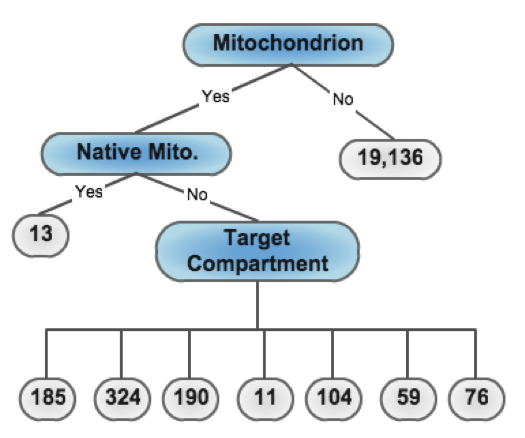
\includegraphics[width=0.75\columnwidth]{fig/Mito_tree}
    \caption{The protein dataset hierarchy of labels along with the instance
    count for each label.}
    \label{fig:Mitotree}
\end{figure}
\FloatBarrier

\section{Coarse-grained vs Fine-grained Trade Off}
\par In hierarchically labeled datasets, over-labeling refers to learning fine-grained
(non-root) concepts and combining the results to predict the coarse-grained (root) label \cite{yugi}.
 It can be demonstrated through a simple example
that for certain datasets, a fine-grained approach to the root level classifier can achieve higher
levels of precision for the same level of recall. Such a dataset is shown in \textit{Figure
\ref{fig:union}}. The classifiers for this dataset can be thought of as a function of axis parallel
rectangular boxes. For the coarse-grained to have high recall and return all of the positive
circle instances, it must encompass the entire dataset
and incidentally return all of the negative diamond instances as
positive also. A fine-grained approach is preferable for the simple dataset pictured. The
fine-grained classification approach for a root
level classifier will achieve higher levels of precision for the same level of recall when
applied to the protein dataset. In the simple example, in order for the coarse-grained learner to have high
    recall, precision must be sacrificed for a large amount of false positives returned.
    By combining fine-grained classifiers, the same level of recall can be achieved with a
    higher level of precision because none of the false positive diamonds will be returned.

\FloatBarrier
\begin{figure}[!htb]
	\centering
    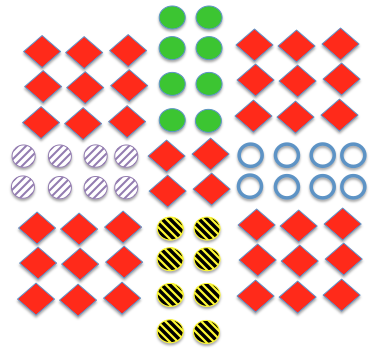
\includegraphics[width=0.5\columnwidth]{fig/union}
    \caption{Demonstration of a dataset that would benefit from multiple fine-grained
    learners for each circle type.}
    \label{fig:union}
\end{figure}
\FloatBarrier


\chapter{Background and Related Work}
\section{Active Learning}
\par Active Learning relates to the coarse-grained vs fine-grained tradeoff because it is
reasonable to assume that fine-grained labels may not be as readily available as coarse-grained
labels, and thus have a higher cost. An active learning approach is used to determine how
many fine-grained labels to purchase in order to minimize the total cost to train the
algorithm an maximize the precision and recall scores. The following equations for
precision, recall, and a weighted F score are shown below in equations 1 through 3.
\break
$Precision eqn$ \break
$Recall eqn$ \break
$F0_5 eqn$ \break
\break
\par The goal in an active learning approach is to maximize the F measure where β equals 0.5 [2].
The F-0.5 measure gives more weight to precision, as opposed to recall, so it gives
incentive to purchase enough fine-grained labels to increase the F-0.5 measure. The
coarse-grained labels will cost less than fine-grained labels, but the increase in
the F-0.5 measure justifies the increase in cost up to a certain point. The F-0.5
measure is used in the results section of this paper. ... That's why we use PR AUC in the results.
Describe some of the other papers that Yugi cited.

\section{Hierarchical Active Learning}
\par The Hierarchical Active Learning algorithm (HAL) is shown diagrammatically in Figure 3.
Multiple fine-grained classifiers are trained at each level of the Hierarchy of the dataset.
Queries to the oracle are performed purchase the most cost effective labels to add to the
training sets of the classifiers. The active learning cycle continues until a cost budget has
been reached. The benefit of an active learning approach is to maximize the F-0.5 measure
for a given cost budget. It was the goal of this study to apply the HAL algorithm to the
protein dataset, however this is not achieved at this time. An existing application of
HAL is briefly discussed in the following section.


\FloatBarrier
\begin{figure}[!htb]
	\centering
    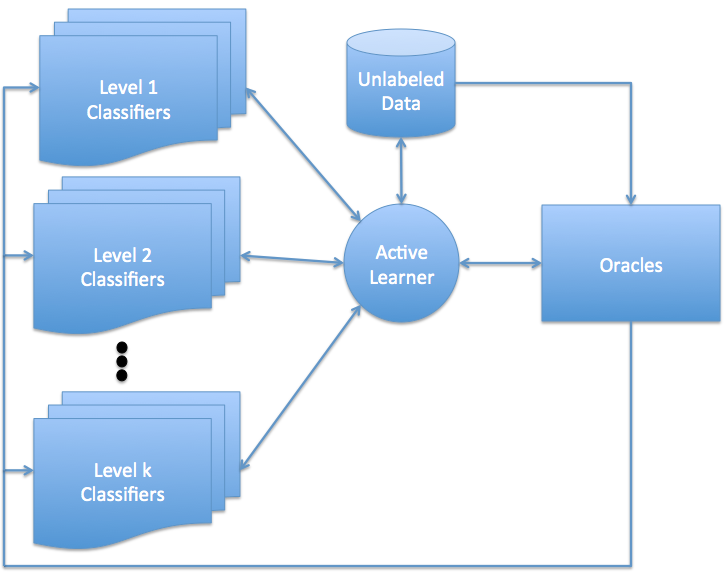
\includegraphics[width=0.5\columnwidth]{fig/AL2}
    \label{fig:AL2}
    \caption{Diagram of HAL approach}
\end{figure}
\FloatBarrier



\section{Application to Dispatch Dataset}
\par HAL was applied to a Dispatch dataset. This dataset contains 375,026 manually labeled
hierarchical names across 1,384 newspaper articles [2]. This is a clear example where
fine-grained labels have a higher cost since it is easier for a person to manually
determine if the article pertains to an organization or not, rather than if it pertains
to a railroad or a zoo, which would be sub labels of the organization root. The first
analysis step was to determine that the F-0.5 measure is increased by using fine-grained classifiers.
The results are shown in Figure 4. The highest F-0.5 measure for
a given iteration of purchases of training instances is obtained by using the active
learning approach with all fine-grained labels. The passive learning curves were
 generated by selecting batches of instances randomly rather than querying the
 oracle for a specific label type that offers that most gain in classifier accuracy.
 The active learning curves did take advantage of querying for specific labels in
 order to maximize gain in classifier accuracy. ... add other data sets.

\FloatBarrier
\begin{figure}[!htb]
	\centering
    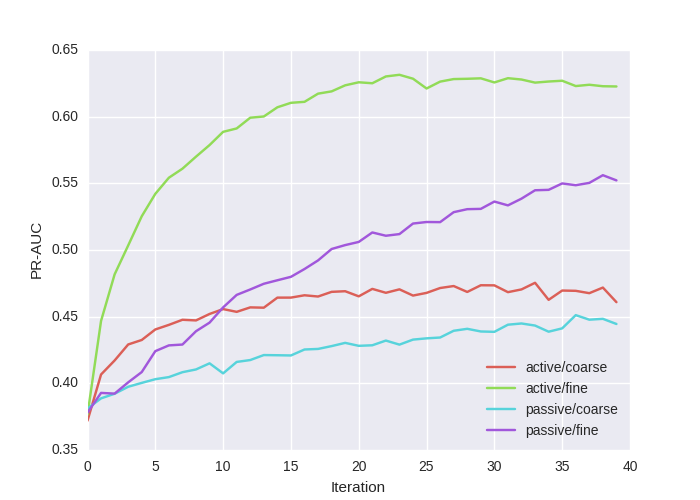
\includegraphics[width=1.0\columnwidth]{fig/draft-richmond}
    \label{fig:draft-richmond}
    \caption{Application of HAL demonstrating the benefit of Actively selecting the type
    of labels to purchase for instances rather than randomly selecting labels to purchase,
    as in the Passive curves.}
\end{figure}
\FloatBarrier


\par The next analysis step is to apply a given ratio of fine-grained vs coarse-grained
labels to purchase at each batch request to the oracle. The results of varying the
percentage of fine-grained labels purchased are shown in Figure 5. The figure shows
that even a small amount of fine-grained labels purchased, that is, 20 precent provides a
significant increase in the F-0.5 measure for a given iteration. ...  PR AUC results.
Add explanation of Bandit approach and results.



\chapter{Experimental Setup}
\section{Training and Testing Coarse Grain and Fine Grain Classifiers}
\par The bioinformatics dataset is composed of 9 classes as shown in
\textit{Figure \ref{fig:Mitotree}}. The coarse-level concept is whether or not
the protein resides within the mitochondria. The negative case of not residing within the mitochondria is class $0$.
The positive case of residing within the
  mitochondria corresponds to any of the $8$ target compartment classes,  numbered $1$ through $8$. Since the
  negative case has no fine-grained labels, the fine-grained classifier is composed of separate classifiers
  for each of the fine-grained labels. The $8$ fine-grained classifiers are trained such that only the instances of
  the class corresponding to that classifier's target compartment are marked as positive, all the others are treated
  as negative. The coarse-level classifier treats all fine-grained target compartment
  instances as members of a single positive class. For all classifiers the non mitochondrion instances are treated as
  negative or $0$ labeled. The totals for each class type is shown in \textit{Table \ref{tab:ClassesAll}}. Throughout
  this experiment a 10 folds cross validation strategy is used, an example partitioning in shown in
  \textit{Table \ref{tab:partitions}}.


\FloatBarrier
\begin{table}[!htb]
\centering
  \caption{This dataset contains 20098 instances total with 449 features each. An example partitioning is shown, some classes
  like 1 and 5 contain only 1-2 instances in a given test set. Note there is a heavy class imbalance with approx. 20 negative
  instances for each positive instance.}
  \label{tab:dataset}
\begin{subtable}{.25\linewidth}
  \centering
  \begin{tabular}{|l||l|}\toprule
    Classes & Count \\ \midrule
    0 & 19136 \\
    1 & 13 \\
    2 & 185 \\
    3 & 324 \\
    4 & 190 \\
    5 & 11 \\
    6 & 104 \\
    7 & 59 \\
    8 & 76 \\ \midrule
    Tot All & 20098 \\
    Tot Coarse & 19136 \\
    Tot Fine & 962 \\
    Features & 449 \\ \bottomrule
  \end{tabular}
  \caption{Classes}
  \label{tab:ClassesAll}
\end{subtable}%
\begin{subtable}{.75\linewidth}
\centering
  \begin{tabular}{|l||l||l||l||l||l||l||l||l||l||l|}\toprule
%    Folds & \multicolumn{9}{c}{Classes} \\ \cmidrule(r){2-11}
    Folds & All & 0 & 1 & 2 & 3 & 4 & 5 & 6 & 7 & 8 \\ \midrule
    1 & 2010 & 1914 & 1 & 19 & 32 & 19 & 1 & 11 & 6 & 7 \\
    2 & 2010 & 1914 & 1 & 19 & 32 & 19 & 1 & 11 & 6 & 7 \\
    3 & 2010 & 1914 & 1 & 19 & 32 & 19 & 1 & 11 & 5 & 8 \\
    4 & 2010 & 1914 & 1 & 19 & 32 & 19 & 1 & 10 & 6 & 8 \\
    5 & 2010 & 1914 & 1 & 18 & 33 & 19 & 1 & 10 & 6 & 8 \\
    6 & 2010 & 1914 & 1 & 18 & 33 & 19 & 1 & 10 & 6 & 8 \\
    7 & 2010 & 1913 & 2 & 18 & 33 & 19 & 1 & 10 & 6 & 8 \\
    8 & 2010 & 1913 & 2 & 18 & 33 & 19 & 1 & 10 & 6 & 8 \\
    9 & 2009 & 1913 & 2 & 18 & 32 & 19 & 2 & 10 & 6 & 7 \\
    10 & 2009 & 1913 & 1 & 19 & 32 & 19 & 1 & 11 & 6 & 7 \\ \midrule
    Total & 20098 & 19136 & 13 & 185 & 324 & 190 & 11 & 104 & 59 & 76 \\
 \bottomrule
  \end{tabular}
  \caption{Folds}
  \label{tab:partitions}
  \end{subtable}
\end{table}
\FloatBarrier



\par Each partition contains a representative portion of each class, the instances are randomly
distributed between partitions. The train set is composed of joining 9 of the partitions together
holding 1 fold out for the test set. An example of the totals for a Train and Test set
is shown on \textit{Table \ref{tab:TrainTest}}.

\FloatBarrier
\begin{table}[H]
  \centering
  \caption{Example of totals for the Train and Test corresponding to when the first fold is
  held out to be the test set.}
  \label{tab:TrainTest}
  \begin{tabular}{|l||l||l||l||l||l||l||l||l||l||l|}\toprule
    Train & All & 0 & 1 & 2 & 3 & 4 & 5 & 6 & 7 & 8 \\
    Total & 18088 & 17222 & 12 & 166 & 292 & 171 & 10 & 93 & 53 & 69 \\ \midrule
    Test & All &  0 & 1 & 2 & 3 & 4 & 5 & 6 & 7 & 8 \\
    Total & 2010 & 1914 & 1 & 19 & 32 & 19 & 1 & 11 & 6 & 7 \\
 \bottomrule
  \end{tabular}
\end{table}
\FloatBarrier

\par Because the experiment will involve running multiple rounds iteratively increasing the
number of instances on which the classifiers are trained and tested, a subset was used to
tune the parameters of the classifiers. This allowed variations of the classifier parameters to be
run rapidly and for the class weight parameter to be tuned for various round sizes. The reduced subset
contains a randomly chosen group of approximately $1/5$ of the negatives. The class totals and example
partitioning for the reduced subset is shown in \textit{Table \ref{tab:subset}}. After tuning parameters
on the subset of data, parameter values are held fixed and experiments are re-run on a new partitioning
containing the entire dataset.

\FloatBarrier
\begin{table}[!htb]
\centering
  \caption{The subset of instances used for tuning classifier parameters contains approximately
  $1/5$ and retains all positive instances.}
  \label{tab:subset}
\begin{subtable}{.25\linewidth}
  \centering
  \begin{tabular}{|l||l|}\toprule
    Classes & Count \\ \midrule
    0 & 3827 \\
    1 & 13 \\
    2 & 185 \\
    3 & 324 \\
    4 & 190 \\
    5 & 11 \\
    6 & 104 \\
    7 & 59 \\
    8 & 76 \\ \midrule
    Tot All & 4789 \\
    Tot Coarse & 3827 \\
    Tot Fine & 962 \\
    Features & 449 \\ \bottomrule
  \end{tabular}
  \caption{Classes Subset}
  \label{tab:ClassesSub}
\end{subtable}%
\begin{subtable}{.75\linewidth}
\centering
  \begin{tabular}{|l||l||l||l||l||l||l||l||l||l||l|}\toprule
    Folds & All & 0 & 1 & 2 & 3 & 4 & 5 & 6 & 7 & 8 \\ \midrule
    1 & 479 & 383 & 1 & 19 & 32 & 19 & 1 & 11 & 6 & 7 \\
    2 & 479 & 383 & 1 & 19 & 32 & 19 & 1 & 11 & 6 & 7 \\
    3 & 479 & 383 & 1 & 19 & 32 & 19 & 1 & 11 & 6 & 7 \\
    4 & 479 & 383 & 1 & 19 & 32 & 19 & 1 & 11 & 5 & 8 \\
    5 & 479 & 383 & 1 & 19 & 32 & 19 & 1 & 10 & 6 & 8 \\
    6 & 479 & 383 & 1 & 18 & 33 & 19 & 1 & 10 & 6 & 8 \\
    7 & 479 & 383 & 1 & 18 & 33 & 19 & 1 & 10 & 6 & 8 \\
    8 & 479 & 382 & 2 & 18 & 33 & 19 & 1 & 10 & 6 & 8 \\
    9 & 479 & 382 & 2 & 18 & 33 & 19 & 1 & 10 & 6 & 8 \\
    10 & 478 & 382 & 2 & 18 & 32 & 19 & 2 & 10 & 6 & 7 \\ \midrule
    Total & 4789 & 3827 & 13 & 185 & 324 & 190 & 11 & 104 & 59 & 76 \\ \bottomrule
  \end{tabular}
  \caption{Folds Subset}
  \label{tab:PartitionsSubset}
  \end{subtable}
\end{table}
\FloatBarrier

\FloatBarrier
\begin{table}[H]
\centering
  \caption{Example totals for the train and test set for the subset of data. The subset of data is
  used for the majority of the parameter search.}
  \label{tab:subTrainTest}
  \begin{tabular}{|l||l||l||l||l||l||l||l||l||l||l|}\toprule
    Train & All & 0 & 1 & 2 & 3 & 4 & 5 & 6 & 7 & 8 \\
    Total & 4310 & 3444 & 12 & 166 & 292 & 171 & 10 & 93 & 53 & 69 \\ \midrule
    Test & All & 0 & 1 & 2 & 3 & 4 & 5 & 6 & 7 & 8 \\
    Total & 479 & 383 & 1 & 19 & 32 & 19 & 1 & 11 & 6 & 7 \\
 \bottomrule
  \end{tabular}
\end{table}
\FloatBarrier


\par Throughout this project the python library sci-kit learn is used for the implementation of the
classification, preprocessing, and evaluation algorithms \cite{scikit-learn}. The Support Vector Machine
(SVM) supervised learning algorithm is used on the un-scaled subset of the data to obtain the base
results shown in \textit{Table \ref{tab:SVMDefResStats}}. The coarse and the fine algorithm performance is shown for each
of the 10 folds along with the average performance across the 10 folds. Also the receiver operator characteristic
and precision recall curves are calculated with fine instances weighted according to the number of of instances in
the test set divided by the number of positive instances in the test set which is a value of 4.99 for the data subset.

\FloatBarrier
\begin{table}[H]
\small
\centering
\caption{SVM default results without parameter selection or preprocessing. Where PR curve AUC
is (pr), ROC curve AUC is (roc), accuracy is (acc), F1-measure is (f1).}
\label{tab:SVMDefResStats}
\begin{tabular}{|l||l||l||l||l||l||l||l|}\toprule
coarse-pr & fine-pr & coarse-roc & fine-roc & coarse-acc & fine-acc & coarse-f1 & fine-f1 \\ \midrule
0.807 & 0.796 & 0.779 & 0.768 & 0.816 & 0.802 & 0.214 & 0.021 \\
0.848 & 0.822 & 0.828 & 0.790 & 0.825 & 0.804 & 0.263 & 0.041 \\
0.846 & 0.821 & 0.810 & 0.765 & 0.818 & 0.802 & 0.243 & 0.021 \\
0.860 & 0.832 & 0.826 & 0.775 & 0.831 & 0.802 & 0.319 & 0.021 \\
0.859 & 0.829 & 0.828 & 0.783 & 0.833 & 0.804 & 0.298 & 0.041 \\
0.796 & 0.763 & 0.748 & 0.715 & 0.816 & 0.806 & 0.214 & 0.061 \\
0.838 & 0.825 & 0.797 & 0.792 & 0.818 & 0.800 & 0.243 & 0.020 \\
0.836 & 0.816 & 0.803 & 0.770 & 0.823 & 0.800 & 0.309 & 0.020 \\
0.863 & 0.845 & 0.833 & 0.805 & 0.829 & 0.797 & 0.305 & 0.000 \\
0.844 & 0.806 & 0.806 & 0.758 & 0.836 & 0.807 & 0.339 & 0.061 \\
avg 0.840 & avg 0.815 & avg 0.806 & avg 0.772 & avg 0.825 & avg 0.802 & avg 0.275 & avg 0.031 \\ \bottomrule
\end{tabular}
\end{table}
\FloatBarrier


\FloatBarrier
\begin{table}[H]
\centering
\caption{SVM default results confusion matrix. Where True Negatives is (tn), False Positives is (fp),
False Negatives (fn), True Positives is (tp).}
\label{tab:SVMDefConfMat}
\begin{tabular}{|l||l||l||l||l||l||l||l|}\toprule
coarse-tn & fine-tn & coarse-fp & fine-fp & coarse-fn & fine-fn & coarse-tp & fine-tp \\ \midrule
379 & 383 & 4 & 0 & 84 & 95 & 12 & 1 \\
380 & 383 & 3 & 0 & 81 & 94 & 15 & 2 \\
378 & 383 & 5 & 0 & 82 & 95 & 14 & 1 \\
379 & 383 & 4 & 0 & 77 & 95 & 19 & 1 \\
382 & 383 & 1 & 0 & 79 & 94 & 17 & 2 \\
379 & 383 & 4 & 0 & 84 & 93 & 12 & 3 \\
378 & 382 & 5 & 1 & 82 & 95 & 14 & 1 \\
375 & 382 & 7 & 0 & 78 & 96 & 19 & 1 \\
379 & 382 & 3 & 0 & 79 & 97 & 18 & 0 \\
379 & 382 & 3 & 0 & 75 & 92 & 20 & 3 \\
avg 378.8 & avg 382.6 & avg 3.9 & avg 0.1 & avg 80.1 & avg 94.6 & avg 16.0 & avg 1.5 \\ \bottomrule
\end{tabular}
\end{table}
\FloatBarrier

\FloatBarrier
\begin{table}[H]
\centering
\caption{SVM default condensed view of summary performance metrics, each value is the average
of 10 folds.}
\label{tab:SVMDef}
\begin{tabular}{|l||l||l||l||l||l||l|}\toprule
title & pr & roc & acc & f1 & conf (tn/fn) & conf (fp/tp) \\ \midrule
coarse & 0.840 & 0.806 & 0.825 & 0.275 & ( 378.8 / 80.1 ) & ( 3.9 / 16.0 ) \\
fine & 0.815 & 0.772 & 0.802 & 0.031 & ( 382.6 / 94.6 ) & ( 0.1 / 1.5 ) \\ \bottomrule
\end{tabular}
\end{table}
\FloatBarrier

\par The primary metric used to make decisions between alternative parameter choices is the PR-AUC and
ROC-AUC. The f-measure and accuracy metrics can be shown to be correlated to a chosen point on the ROC or
PR curves. As shown in \textit{Figure \ref{fig:LogRegThreshAcc}} on \textit{page \pageref{fig:LogRegThreshAcc}},
each point on the ROC curve has an associated chosen accuracy point, both the coarse and fine classifiers have similar
sets of accuracy and f-measure points. The chosen threshold used to output the accuracy, f-measure and confusion matrices
varies between the coarse and fine classifier, so at a first glance it appears as if fine out performs coarse in these
metrics but an alternative threshold could be selected for the coarse classifier to obtain metrics matching the fine
output. Alternatively, the PR-AUC and ROC-AUC compare the correctness of the entire ranking of the
instances in the test set by the classifier, and thus eliminate the need to consider the dynamic tuning of the threshold
used by the classifier to output a given confusion matrix, accuracy, and f-measure score.



\subsection{Varying SVM Scaling Methods}
\par Different scaling methods were used to preprocess the data \cite{scikit-learn}. The standard scaling (std-scaler) strategy
centers all features around zero and have variance in the same order, it outputs the features with a mean of zero
and a unit variance. The minimum maximum scaling (minimax-scaler) strategy scales features between a minimum and maximum value,
which is 0 and 1. The normalization scaling (norm-scaler) strategy scales individual samples to have a unit norm. Each
preprocessing strategy is applied on the entire dataset before training and testing is performed. Preprocessing was performed
with a radial basis function kernel.

\FloatBarrier

\begin{table}[H]
\centering
\caption{SVM minimax-scaler results.}
\label{tab:SVMMinMax}
\begin{tabular}{|l||l||l||l||l||l||l|}\toprule
title & pr & roc & acc & f1 & conf (tn/fn) & conf (fp/tp) \\ \midrule
coarse & 0.881 & 0.855 & 0.799 & 0.000 & ( 382.7 / 96.1 ) & ( 0.0 / 0.0 ) \\
fine & 0.840 & 0.810 & 0.799 & 0.000 & ( 382.7 / 96.1 ) & ( 0.0 / 0.0 ) \\ \bottomrule
\end{tabular}
\end{table}
\FloatBarrier


\FloatBarrier
\begin{table}[H]
\centering
\caption{SVM norm-scaler results.}
\label{tab:SVMNorm}
\begin{tabular}{|l||l||l||l||l||l||l|}\toprule
title & pr & roc & acc & f1 & conf (tn/fn) & conf (fp/tp) \\ \midrule
coarse & 0.801 & 0.791 & 0.799 & 0.000 & ( 382.7 / 96.1 ) & ( 0.0 / 0.0 ) \\
fine & 0.636 & 0.615 & 0.799 & 0.000 & ( 382.7 / 96.1 ) & ( 0.0 / 0.0 ) \\ \bottomrule
\end{tabular}
\end{table}
\FloatBarrier

\FloatBarrier
\begin{table}[H]
\centering
\caption{SVM std-scaler results. This option is chosen.}
\label{tab:SVMStandard}
\begin{tabular}{|l||l||l||l||l||l||l|}\toprule
title & pr & roc & acc & f1 & conf (tn/fn) & conf (fp/tp) \\ \midrule
coarse & 0.912 & 0.882 & 0.881 & 0.631 & ( 372.7 / 47.1 ) & ( 10.0 / 49.0 ) \\
fine & 0.879 & 0.848 & 0.809 & 0.094 & ( 382.7 / 91.3 ) & ( 0.0 / 4.8 ) \\ \bottomrule
\end{tabular}
\end{table}
\FloatBarrier


\subsection{Varying SVM Kernels}
\par Different kernel functions were used in the SVM classifier including: Radial Basis Function (RBF), Polynomial
Degree 3 and 6 (Poly), Linear, and Sigmoid \cite{scikit-learn}. The chosen preprocessing strategy of
std-scaler is used for these results. As parameter selection is elicited the choices from previous sections
are used in any sections that follow.



\FloatBarrier
\begin{table}[H]
\centering
\caption{Linear kernel results.}
\label{tab:Linear}
\begin{tabular}{|l||l||l||l||l||l||l|}\toprule
title & pr & roc & acc & f1 & conf (tn/fn) & conf (fp/tp) \\ \midrule
coarse & 0.867 & 0.841 & 0.853 & 0.599 & ( 355.5 / 43.4 ) & ( 27.2 / 52.7 ) \\
fine & 0.816 & 0.789 & 0.828 & 0.523 & ( 351.1 / 50.8 ) & ( 31.6 / 45.3 ) \\ \bottomrule
\end{tabular}
\end{table}
\FloatBarrier

\FloatBarrier
\begin{table}[H]
\centering
\caption{Poly degree 3 kernel results.}
\label{tab:polyDeg3}
\begin{tabular}{|l||l||l||l||l||l||l|}\toprule
title & pr & roc & acc & f1 & conf (tn/fn) & conf (fp/tp) \\ \midrule
coarse & 0.816 & 0.817 & 0.807 & 0.169 & ( 376.9 / 86.7 ) & ( 5.8 / 9.4 ) \\
fine & 0.755 & 0.743 & 0.801 & 0.063 & ( 380.3 / 92.9 ) & ( 2.3 / 3.2 ) \\ \bottomrule
\end{tabular}
\end{table}
\FloatBarrier

\FloatBarrier
\begin{table}[H]
\centering
\caption{Poly degree 6 kernel results.}
\label{tab:polyDeg6}
\begin{tabular}{|l||l||l||l||l||l||l|}\toprule
title & pr & roc & acc & f1 & conf (tn/fn) & conf (fp/tp) \\ \midrule
coarse & 0.659 & 0.637 & 0.797 & 0.037 & ( 379.5 / 94.2 ) & ( 3.2 / 1.9 ) \\
fine & 0.624 & 0.584 & 0.794 & 0.020 & ( 379.0 / 95.1 ) & ( 3.7 / 1.0 ) \\ \bottomrule
\end{tabular}
\end{table}
\FloatBarrier

\FloatBarrier
\begin{table}[H]
\centering
\caption{Sigmoid kernel results.}
\label{tab:sigmoid}
\begin{tabular}{|l||l||l||l||l||l||l|}\toprule
title & pr & roc & acc & f1 & conf (tn/fn) & conf (fp/tp) \\ \midrule
coarse & 0.703 & 0.693 & 0.773 & 0.405 & ( 333.0 / 59.0 ) & ( 49.7 / 37.1 ) \\
fine & 0.653 & 0.622 & 0.789 & 0.127 & ( 370.3 / 88.7 ) & ( 12.4 / 7.4 ) \\ \bottomrule
\end{tabular}
\end{table}
\FloatBarrier

\FloatBarrier
\begin{table}[H]
\centering
\caption{RBF kernel results. This option is chosen.}
\label{tab:RbfOrig}
\begin{tabular}{|l||l||l||l||l||l||l|}\toprule
title & pr & roc & acc & f1 & conf (tn/fn) & conf (fp/tp) \\ \midrule
coarse & 0.912 & 0.882 & 0.881 & 0.630 & ( 372.6 / 47.1 ) & ( 10.1 / 49.0 ) \\
fine & 0.879 & 0.848 & 0.809 & 0.094 & ( 382.7 / 91.3 ) & ( 0.0 / 4.8 ) \\ \bottomrule
\end{tabular}
\end{table}
\FloatBarrier

\subsection{Varying SVM Feature Selection}
\par I tried different feature selection percentages. The Select Percentile library was used from
sci-kit learn \cite{scikit-learn}. This is a univariate feature selection strategy that ranks the
features usability for classification according to a statistical measure, then keeps a certain
percentage of the features. The 100\% example is the option chosen in the previous section.

\FloatBarrier
\begin{table}[H]
\centering
\caption{SVM select percentile, keep 25\% of features.}
\label{tab:SVMSel25}
\begin{tabular}{|l||l||l||l||l||l||l|}\toprule
title & pr & roc & acc & f1 & conf (tn/fn) & conf (fp/tp) \\ \midrule
coarse & 0.907 & 0.875 & 0.877 & 0.623 & ( 370.7 / 47.1 ) & ( 12.0 / 49.0 ) \\
fine & 0.854 & 0.823 & 0.806 & 0.068 & ( 382.7 / 92.7 ) & ( 0.0 / 3.4 ) \\ \bottomrule
\end{tabular}
\end{table}
\FloatBarrier


\FloatBarrier
\begin{table}[H]
\centering
\caption{SVM select percentile, keep 50\% of features.}
\label{tab:SVMSel50}
\begin{tabular}{|l||l||l||l||l||l||l|}\toprule
title & pr & roc & acc & f1 & conf (tn/fn) & conf (fp/tp) \\ \midrule
coarse & 0.913 & 0.885 & 0.879 & 0.632 & ( 371.3 / 46.4 ) & ( 11.4 / 49.7 ) \\
fine & 0.874 & 0.842 & 0.810 & 0.097 & ( 382.7 / 91.2 ) & ( 0.0 / 4.9 ) \\ \bottomrule
\end{tabular}
\end{table}
\FloatBarrier



\FloatBarrier
\begin{table}[H]
\centering
\caption{SVM select percentile, keep 75\% of features. This option is chosen.}
\label{tab:SVMSel75}
\begin{tabular}{|l||l||l||l||l||l||l|}\toprule
title & pr & roc & acc & f1 & conf (tn/fn) & conf (fp/tp) \\ \midrule
coarse & 0.913 & 0.883 & 0.878 & 0.622 & ( 372.1 / 47.9 ) & ( 10.6 / 48.2 ) \\
fine & 0.880 & 0.848 & 0.809 & 0.089 & ( 382.7 / 91.6 ) & ( 0.0 / 4.5 ) \\ \bottomrule
\end{tabular}
\end{table}
\FloatBarrier

\par Note that leveraging the fine-grained labels did not improve classifier performance
relative to the coarse classifier. An alternative classifier strategy Logistic Regression
 (Logit) is investigated.


\subsection{Varying Logistic Regression Scaling}
\par Tested out the same options for preprocessing scaling, that were varied for SVM.

\FloatBarrier
\begin{table}[H]
\centering
\caption{Logistic Regression - No scaling.}
\label{tab:LogRegDef}
\begin{tabular}{|l||l||l||l||l||l||l|}\toprule
title & pr & roc & acc & f1 & conf (tn/fn) & conf (fp/tp) \\ \midrule
coarse & 0.887 & 0.862 & 0.867 & 0.615 & ( 364.1 / 45.0 ) & ( 18.6 / 51.1 ) \\
fine & 0.854 & 0.837 & 0.833 & 0.395 & ( 372.8 / 69.9 ) & ( 9.9 / 26.2 ) \\ \bottomrule
\end{tabular}
\end{table}
\FloatBarrier

\FloatBarrier
\begin{table}[H]
\centering
\caption{Logistic Regression standard scaling.}
\label{tab:LogRegStandard}
\begin{tabular}{|l||l||l||l||l||l||l|}\toprule
title & pr & roc & acc & f1 & conf (tn/fn) & conf (fp/tp) \\ \midrule
coarse & 0.864 & 0.849 & 0.846 & 0.583 & ( 353.8 / 44.8 ) & ( 28.7 / 51.3 ) \\
fine & 0.833 & 0.816 & 0.831 & 0.471 & ( 362.0 / 60.2 ) & ( 20.5 / 36.0 ) \\ \bottomrule
\end{tabular}
\end{table}
\FloatBarrier

\FloatBarrier
\begin{table}[H]
\centering
\caption{Logistic Regression normalization scaling.}
\label{tab:LogRegNorm}
\begin{tabular}{|l||l||l||l||l||l||l|}\toprule
title & pr & roc & acc & f1 & conf (tn/fn) & conf (fp/tp) \\ \midrule
coarse & 0.790 & 0.761 & 0.799 & 0.000 & ( 382.7 / 96.1 ) & ( 0.0 / 0.0 ) \\
fine & 0.767 & 0.735 & 0.799 & 0.000 & ( 382.7 / 96.1 ) & ( 0.0 / 0.0 ) \\ \bottomrule
\end{tabular}
\end{table}
\FloatBarrier

\FloatBarrier
\begin{table}[H]
\centering
\caption{Logistic Regression MinMax scaling. This option is chosen.}
\label{tab:LogRegMinMax}
\begin{tabular}{|l||l||l||l||l||l||l|}\toprule
title & pr & roc & acc & f1 & conf (tn/fn) & conf (fp/tp) \\ \midrule
coarse & 0.891 & 0.867 & 0.864 & 0.581 & ( 368.6 / 50.9 ) & ( 14.1 / 45.2 ) \\
fine & 0.888 & 0.862 & 0.812 & 0.130 & ( 382.1 / 89.3 ) & ( 0.6 / 6.8 ) \\ \bottomrule
\end{tabular}
\end{table}
\FloatBarrier


\subsection{Varying Logistic Regression Feature Selection}
\par Tested out the same options for feature selection that were varied for SVM.

\FloatBarrier
\begin{table}[H]
\centering
\caption{Logistic Regression select percentile 25\%.}
\label{tab:LogRegSel25}
\begin{tabular}{|l||l||l||l||l||l||l|}\toprule
title & pr & roc & acc & f1 & conf (tn/fn) & conf (fp/tp) \\ \midrule
coarse & 0.872 & 0.848 & 0.849 & 0.497 & ( 370.8 / 60.3 ) & ( 11.9 / 35.8 ) \\
fine & 0.869 & 0.845 & 0.804 & 0.052 & ( 382.2 / 93.5 ) & ( 0.5 / 2.6 ) \\ \bottomrule
\end{tabular}
\end{table}
\FloatBarrier


\FloatBarrier
\begin{table}[H]
\centering
\caption{Logistic Regression select percentile 50\%.}
\label{tab:LogRegSel50}
\begin{tabular}{|l||l||l||l||l||l||l|}\toprule
title & pr & roc & acc & f1 & conf (tn/fn) & conf (fp/tp) \\ \midrule
coarse & 0.875 & 0.849 & 0.849 & 0.497 & ( 370.8 / 60.3 ) & ( 11.9 / 35.8 ) \\
fine & 0.872 & 0.846 & 0.803 & 0.050 & ( 382.2 / 93.6 ) & ( 0.5 / 2.5 ) \\ \bottomrule
\end{tabular}
\end{table}
\FloatBarrier

\FloatBarrier
\begin{table}[H]
\centering
\caption{Logistic Regression select percentile 75\%.}
\label{tab:LogRegSel75}
\begin{tabular}{|l||l||l||l||l||l||l|}\toprule
title & pr & roc & acc & f1 & conf (tn/fn) & conf (fp/tp) \\ \midrule
coarse & 0.871 & 0.847 & 0.848 & 0.493 & ( 370.6 / 60.6 ) & ( 12.1 / 35.5 ) \\
fine & 0.869 & 0.845 & 0.803 & 0.048 & ( 382.0 / 93.7 ) & ( 0.7 / 2.4 ) \\ \bottomrule
\end{tabular}
\end{table}
\FloatBarrier


\FloatBarrier
\begin{table}[H]
\centering
\caption{Logistic Regression select percentile 100\%. This option is chosen.}
\label{tab:LogRegMinMax}
\begin{tabular}{|l||l||l||l||l||l||l|}\toprule
title & pr & roc & acc & f1 & conf (tn/fn) & conf (fp/tp) \\ \midrule
coarse & 0.891 & 0.867 & 0.864 & 0.581 & ( 368.6 / 50.9 ) & ( 14.1 / 45.2 ) \\
fine & 0.888 & 0.862 & 0.812 & 0.130 & ( 382.1 / 89.3 ) & ( 0.6 / 6.8 ) \\ \bottomrule
\end{tabular}
\end{table}
\FloatBarrier


\subsection{Varying Logistic Regression Positive Class Weight and Cost}
\par Since there is a class imbalance in the dataset, see \textit{Table \ref{tab:ClassesAll} } on
\textit{page \pageref{tab:ClassesAll}}, class weight and cost parameter pairs are varied.  The cost
default value is 1.0, and the class weight default value is 1.0. The original value for weighting the
fine training instance is the number of instances in the train set divided by the number of positive
instances, this is 4.977. The negative instance train weight is always 1.0.

\FloatBarrier
\begin{table}[H]
\centering
\caption{Logit weight 4.977, cost 1.0}
\label{tab:LogRegWtOrig-C1}
\begin{tabular}{|l||l||l||l||l||l||l|}\toprule
title & pr & roc & acc & f1 & conf (tn/fn) & conf (fp/tp) \\ \midrule
coarse & 0.886 & 0.868 & 0.787 & 0.606 & ( 298.7 / 17.9 ) & ( 84.0 / 78.2 ) \\
fine & 0.885 & 0.862 & 0.857 & 0.587 & ( 361.7 / 47.3 ) & ( 21.0 / 48.8 ) \\ \bottomrule
\end{tabular}
\end{table}
\FloatBarrier

\FloatBarrier
\begin{table}[H]
\centering
\caption{Logit weight 4.977, cost 0.1}
\label{tab:LogRegWtOrig-Cp1}
\begin{tabular}{|l||l||l||l||l||l||l|}\toprule
title & pr & roc & acc & f1 & conf (tn/fn) & conf (fp/tp) \\ \midrule
coarse & 0.880 & 0.861 & 0.755 & 0.579 & ( 280.7 / 15.4 ) & ( 102.0 / 80.7 ) \\
fine & 0.880 & 0.856 & 0.851 & 0.483 & ( 374.2 / 62.7 ) & ( 8.5 / 33.4 ) \\ \bottomrule
\end{tabular}
\end{table}
\FloatBarrier


\FloatBarrier
\begin{table}[H]
\centering
\caption{Logit weight 4.977, cost 10.0}
\label{tab:LogRegWtOrig-C10}
\begin{tabular}{|l||l||l||l||l||l||l|}\toprule
title & pr & roc & acc & f1 & conf (tn/fn) & conf (fp/tp) \\ \midrule
coarse & 0.876 & 0.855 & 0.793 & 0.603 & ( 304.6 / 21.1 ) & ( 78.1 / 75.0 ) \\
fine & 0.866 & 0.842 & 0.835 & 0.583 & ( 344.8 / 40.9 ) & ( 37.9 / 55.2 ) \\ \bottomrule
\end{tabular}
\end{table}
\FloatBarrier


\FloatBarrier
\begin{table}[H]
\centering
\caption{Logit weight 10.0, cost 1.0}
\label{tab:LogRegWt10-C1}
\begin{tabular}{|l||l||l||l||l||l||l|}\toprule
title & pr & roc & acc & f1 & conf (tn/fn) & conf (fp/tp) \\ \midrule
coarse & 0.883 & 0.865 & 0.690 & 0.536 & ( 245.4 / 10.9 ) & ( 137.3 / 85.2 ) \\
fine & 0.880 & 0.859 & 0.822 & 0.620 & ( 324.2 / 26.7 ) & ( 58.5 / 69.4 ) \\ \bottomrule
\end{tabular}
\end{table}
\FloatBarrier


\FloatBarrier
\begin{table}[H]
\centering
\caption{Logit weight 10.0, cost 0.1}
\label{tab:LogRegWt10-Cp1}
\begin{tabular}{|l||l||l||l||l||l||l|}\toprule
title & pr & roc & acc & f1 & conf (tn/fn) & conf (fp/tp) \\ \midrule
coarse & 0.879 & 0.863 & 0.609 & 0.486 & ( 203.6 / 7.9 ) & ( 179.1 / 88.2 ) \\
fine & 0.881 & 0.859 & 0.834 & 0.621 & ( 334.5 / 31.1 ) & ( 48.2 / 65.0 ) \\ \bottomrule
\end{tabular}
\end{table}
\FloatBarrier

\FloatBarrier
\begin{table}[H]
\centering
\caption{Logit weight 10.0, cost 10.0}
\label{tab:LogRegWt10-C10}
\begin{tabular}{|l||l||l||l||l||l||l|}\toprule
title & pr & roc & acc & f1 & conf (tn/fn) & conf (fp/tp) \\ \midrule
coarse & 0.871 & 0.851 & 0.723 & 0.554 & ( 264.1 / 13.9 ) & ( 118.6 / 82.2 ) \\
fine & 0.861 & 0.837 & 0.792 & 0.585 & ( 309.3 / 26.2 ) & ( 73.4 / 69.9 ) \\ \bottomrule
\end{tabular}
\end{table}
\FloatBarrier

\FloatBarrier
\begin{table}[H]
\centering
\caption{Logit weight 7.5, cost 1.0}
\label{tab:LogRegWt7p5-C1}
\begin{tabular}{|l||l||l||l||l||l||l|}\toprule
title & pr & roc & acc & f1 & conf (tn/fn) & conf (fp/tp) \\ \midrule
coarse & 0.884 & 0.867 & 0.734 & 0.566 & ( 268.8 / 13.5 ) & ( 113.9 / 82.6 ) \\
fine & 0.882 & 0.861 & 0.846 & 0.624 & ( 343.4 / 34.6 ) & ( 39.3 / 61.5 ) \\ \bottomrule
\end{tabular}
\end{table}
\FloatBarrier

\FloatBarrier
\begin{table}[H]
\centering
\caption{Logit weight 7.5, cost 0.1. This option is chosen due to showing advantage for the
fine classifier compared to the coarse classifier.}
\label{tab:LogRegWt7p5-Cp1}
\begin{tabular}{|l||l||l||l||l||l||l|}\toprule
title & pr & roc & acc & f1 & conf (tn/fn) & conf (fp/tp) \\ \midrule
coarse & 0.880 & 0.862 & 0.668 & 0.517 & ( 234.8 / 11.1 ) & ( 147.9 / 85.0 ) \\
fine & 0.881 & 0.858 & 0.859 & 0.613 & ( 357.3 / 42.3 ) & ( 25.4 / 53.8 ) \\ \bottomrule
\end{tabular}
\end{table}
\FloatBarrier

\FloatBarrier
\begin{table}[H]
\centering
\caption{Logit weight 7.5, cost 10.0}
\label{tab:LogRegWt7p5-C10}
\begin{tabular}{|l||l||l||l||l||l||l|}\toprule
title & pr & roc & acc & f1 & conf (tn/fn) & conf (fp/tp) \\ \midrule
coarse & 0.873 & 0.852 & 0.757 & 0.578 & ( 283.2 / 16.7 ) & ( 99.5 / 79.4 ) \\
fine & 0.863 & 0.839 & 0.810 & 0.588 & ( 323.3 / 31.4 ) & ( 59.4 / 64.7 ) \\ \bottomrule
\end{tabular}
\end{table}
\FloatBarrier



\subsection{Varying Logistic Regression Fine Class Weights}
\par The weight for each of the separate fine classes is tuned by multiplying,
the class weight of 7.5, determined in the previous section by a fixed ratio. A
weight ratio of 1.0 would output a fine class weight of 7.5. A weight ratio of
 0.5 would output a fine class weight of 3.75. Subsections showing the tuning results
 for each of the 8 fine-grained classes follow. The confusion matrices and output metrics for the individual
 fine class are shown in order to demonstrate how well the classifier is learning that
 fine-grained class. These metrics are the average of 10 folds. The coarse classifier output
 is not shown as it will not vary or be dependent upon the fine class weight tuning.

\subsubsection{Tune Fine Class 1 Weights}
\FloatBarrier
\begin{table}[H]
\centering
\caption{Logit Class 1 weight ratio 1.0}
\label{tab:LogRegCls1-Wt1}
\begin{tabular}{|l||l||l||l||l||l||l|}\toprule
title & pr & roc & acc & f1 & conf (tn/fn) & conf (fp/tp) \\ \midrule
fine & 0.881 & 0.858 & 0.859 & 0.613 & ( 357.3 / 42.3 ) & ( 25.4 / 53.8 ) \\
trainCls-1 & 0.995 & 0.999 & 0.998 & 0.477 & ( 4297.7 / 7.7 ) & ( 0.8 / 4.0 ) \\
testCls-1 & 0.722 & 0.996 & 0.997 & 0.100 & ( 477.4 / 1.2 ) & ( 0.1 / 0.1 ) \\ \bottomrule
\end{tabular}
\end{table}
\FloatBarrier


\FloatBarrier
\begin{table}[H]
\centering
\caption{Logit Class 1 weight ratio 0.5}
\label{tab:LogRegCls1-Wtp5}
\begin{tabular}{|l||l||l||l||l||l||l|}\toprule
title & pr & roc & acc & f1 & conf (tn/fn) & conf (fp/tp) \\ \midrule
fine & 0.880 & 0.856 & 0.859 & 0.613 & ( 357.4 / 42.3 ) & ( 25.3 / 53.8 ) \\
trainCls-1 & 0.994 & 0.998 & 0.997 & 0.142 & ( 4298.5 / 10.8 ) & ( 0.0 / 0.9 ) \\
testCls-1 & 0.696 & 0.995 & 0.997 & 0.000 & ( 477.5 / 1.3 ) & ( 0.0 / 0.0 ) \\ \bottomrule
\end{tabular}
\end{table}
\FloatBarrier

\FloatBarrier
\begin{table}[H]
\centering
\caption{Logit Class 1 weight ratio 3.0. This option is chosen.}
\label{tab:LogRegCls1-Wt3}
\begin{tabular}{|l||l||l||l||l||l||l|}\toprule
title & pr & roc & acc & f1 & conf (tn/fn) & conf (fp/tp) \\ \midrule
fine & 0.882 & 0.860 & 0.859 & 0.617 & ( 357.1 / 41.7 ) & ( 25.6 / 54.4 ) \\
trainCls-1 & 0.995 & 1.000 & 0.999 & 0.854 & ( 4295.8 / 1.0 ) & ( 2.7 / 10.7 ) \\
testCls-1 & 0.722 & 0.997 & 0.998 & 0.400 & ( 477.1 / 0.7 ) & ( 0.4 / 0.6 ) \\ \bottomrule
\end{tabular}
\end{table}
\FloatBarrier

\FloatBarrier
\begin{table}[H]
\centering
\caption{Logit Class 1 weight ratio 5.0}
\label{tab:LogRegCls1-Wt5}
\begin{tabular}{|l||l||l||l||l||l||l|}\toprule
title & pr & roc & acc & f1 & conf (tn/fn) & conf (fp/tp) \\ \midrule
fine & 0.881 & 0.859 & 0.860 & 0.618 & ( 357.0 / 41.5 ) & ( 25.7 / 54.6 ) \\
trainCls-1 & 0.995 & 1.000 & 0.999 & 0.850 & ( 4294.3 / 0.0 ) & ( 4.2 / 11.7 ) \\
testCls-1 & 0.722 & 0.997 & 0.998 & 0.513 & ( 476.9 / 0.5 ) & ( 0.6 / 0.8 ) \\ \bottomrule
\end{tabular}
\end{table}
\FloatBarrier


\subsubsection{Tune Fine Class 2 Weights}
\FloatBarrier
\begin{table}[H]
\centering
\caption{Logit Class 2 weight ratio 1.0. This option is chosen.}
\label{tab:LogRegCls2-Wt1}
\begin{tabular}{|l||l||l||l||l||l||l|}\toprule
title & pr & roc & acc & f1 & conf (tn/fn) & conf (fp/tp) \\ \midrule
fine & 0.882 & 0.860 & 0.859 & 0.617 & ( 357.1 / 41.7 ) & ( 25.6 / 54.4 ) \\
trainCls-2 & 0.800 & 0.804 & 0.952 & 0.200 & ( 4076.9 / 140.5 ) & ( 66.8 / 26.0 ) \\
testCls-2 & 0.655 & 0.689 & 0.944 & 0.081 & ( 450.7 / 17.3 ) & ( 9.6 / 1.2 ) \\ \bottomrule
\end{tabular}
\end{table}
\FloatBarrier

\FloatBarrier
\begin{table}[H]
\centering
\caption{Logit Class 2 weight ratio 0.5}
\label{tab:LogitCls2-Wtp5}
\begin{tabular}{|l||l||l||l||l||l||l|}\toprule
title & pr & roc & acc & f1 & conf (tn/fn) & conf (fp/tp) \\ \midrule
fine & 0.882 & 0.857 & 0.862 & 0.618 & ( 359.1 / 42.5 ) & ( 23.6 / 53.6 ) \\
trainCls-2 & 0.785 & 0.787 & 0.961 & 0.052 & ( 4139.4 / 161.9 ) & ( 4.3 / 4.6 ) \\
testCls-2 & 0.656 & 0.694 & 0.960 & 0.009 & ( 459.4 / 18.4 ) & ( 0.9 / 0.1 ) \\ \bottomrule
\end{tabular}
\end{table}
\FloatBarrier

\FloatBarrier
\begin{table}[H]
\centering
\caption{Logit Class 2 weight ratio 1.5}
\label{tab:LogRegCls2-Wt1p5}
\begin{tabular}{|l||l||l||l||l||l||l|}\toprule
title & pr & roc & acc & f1 & conf (tn/fn) & conf (fp/tp) \\ \midrule
fine & 0.877 & 0.857 & 0.855 & 0.620 & ( 352.5 / 39.3 ) & ( 30.2 / 56.8 ) \\
trainCls-2 & 0.806 & 0.814 & 0.924 & 0.263 & ( 3924.1 / 108.1 ) & ( 219.6 / 58.4 ) \\
testCls-2 & 0.652 & 0.684 & 0.914 & 0.123 & ( 434.8 / 15.6 ) & ( 25.5 / 2.9 ) \\ \bottomrule
\end{tabular}
\end{table}
\FloatBarrier


\subsubsection{Tune Fine Class 3 Weights}
\FloatBarrier
\begin{table}[H]
\centering
\caption{Logit Class 3 weight ratio 1.0. This option is chosen.}
\label{tab:LogRegCls3-Wt1}
\begin{tabular}{|l||l||l||l||l||l||l|}\toprule
title & pr & roc & acc & f1 & conf (tn/fn) & conf (fp/tp) \\ \midrule
fine & 0.882 & 0.860 & 0.859 & 0.617 & ( 357.1 / 41.7 ) & ( 25.6 / 54.4 ) \\
trainCls-3 & 0.846 & 0.852 & 0.882 & 0.401 & ( 3628.6 / 120.7 ) & ( 390.0 / 170.9 ) \\
testCls-3 & 0.795 & 0.803 & 0.873 & 0.360 & ( 401.2 / 15.4 ) & ( 45.2 / 17.0 ) \\ \bottomrule
\end{tabular}
\end{table}
\FloatBarrier


\FloatBarrier
\begin{table}[H]
\centering
\caption{Logit Class 3 weight ratio 0.5}
\label{tab:LogRegCls3-Wtp5}
\begin{tabular}{|l||l||l||l||l||l||l|}\toprule
title & pr & roc & acc & f1 & conf (tn/fn) & conf (fp/tp) \\ \midrule
fine & 0.870 & 0.852 & 0.839 & 0.445 & ( 370.9 / 65.1 ) & ( 11.8 / 31.0 ) \\
trainCls-3 & 0.838 & 0.838 & 0.929 & 0.288 & ( 3942.0 / 229.7 ) & ( 76.6 / 61.9 ) \\
testCls-3 & 0.792 & 0.798 & 0.925 & 0.246 & ( 437.2 / 26.5 ) & ( 9.2 / 5.9 ) \\ \bottomrule
\end{tabular}
\end{table}
\FloatBarrier

\FloatBarrier
\begin{table}[H]
\centering
\caption{Logit Class 3 weight ratio 1.5}
\label{tab:LogRegCls3-Wt1p5}
\begin{tabular}{|l||l||l||l||l||l||l|}\toprule
title & pr & roc & acc & f1 & conf (tn/fn) & conf (fp/tp) \\ \midrule
fine & 0.879 & 0.855 & 0.832 & 0.626 & ( 331.2 / 28.9 ) & ( 51.5 / 67.2 ) \\
trainCls-3 & 0.849 & 0.859 & 0.813 & 0.351 & ( 3288.4 / 74.5 ) & ( 730.2 / 217.1 ) \\
testCls-3 & 0.795 & 0.805 & 0.804 & 0.318 & ( 363.3 / 10.6 ) & ( 83.1 / 21.8 ) \\ \bottomrule
\end{tabular}
\end{table}
\FloatBarrier


\subsubsection{Tune Fine Class 4 Weights}
\FloatBarrier
\begin{table}[H]
\centering
\caption{Logit Class 4 weight ratio 1.0}
\label{tab:LogRegCls4-Wt1}
\begin{tabular}{|l||l||l||l||l||l||l|}\toprule
title & pr & roc & acc & f1 & conf (tn/fn) & conf (fp/tp) \\ \midrule
fine & 0.882 & 0.860 & 0.859 & 0.617 & ( 357.1 / 41.7 ) & ( 25.6 / 54.4 ) \\
trainCls-4 & 0.937 & 0.942 & 0.960 & 0.531 & ( 4038.6 / 72.9 ) & ( 100.6 / 98.1 ) \\
testCls-4 & 0.882 & 0.902 & 0.952 & 0.433 & ( 447.1 / 10.2 ) & ( 12.7 / 8.8 ) \\ \bottomrule
\end{tabular}
\end{table}
\FloatBarrier

\FloatBarrier
\begin{table}[H]
\centering
\caption{Logit Class 4 weight ratio 0.5}
\label{tab:LogRegCls4-Wtp5}
\begin{tabular}{|l||l||l||l||l||l||l|}\toprule
title & pr & roc & acc & f1 & conf (tn/fn) & conf (fp/tp) \\ \midrule
fine & 0.875 & 0.852 & 0.855 & 0.590 & ( 359.2 / 45.9 ) & ( 23.5 / 50.2 ) \\
trainCls-4 & 0.928 & 0.932 & 0.965 & 0.397 & ( 4108.1 / 120.9 ) & ( 31.1 / 50.1 ) \\
testCls-4 & 0.878 & 0.898 & 0.962 & 0.320 & ( 456.0 / 14.6 ) & ( 3.8 / 4.4 ) \\ \bottomrule
\end{tabular}
\end{table}
\FloatBarrier


\FloatBarrier
\begin{table}[H]
\centering
\caption{Logit Class 4 weight ratio 1.5. This option is chosen.}
\label{tab:LogRegCls4-Wt1p5}
\begin{tabular}{|l||l||l||l||l||l||l|}\toprule
title & pr & roc & acc & f1 & conf (tn/fn) & conf (fp/tp) \\ \midrule
fine & 0.883 & 0.861 & 0.856 & 0.624 & ( 352.4 / 38.8 ) & ( 30.3 / 57.3 ) \\
trainCls-4 & 0.941 & 0.947 & 0.936 & 0.462 & ( 3918.1 / 53.2 ) & ( 221.1 / 117.8 ) \\
testCls-4 & 0.886 & 0.903 & 0.926 & 0.382 & ( 432.5 / 8.0 ) & ( 27.3 / 11.0 ) \\ \bottomrule
\end{tabular}
\end{table}
\FloatBarrier

\FloatBarrier
\begin{table}[H]
\centering
\caption{Logit Class 4 weight ratio 2.0}
\label{tab:LogRegCls4-Wt2}
\begin{tabular}{|l||l||l||l||l||l||l|}\toprule
title & pr & roc & acc & f1 & conf (tn/fn) & conf (fp/tp) \\ \midrule
fine & 0.880 & 0.859 & 0.853 & 0.627 & ( 348.9 / 36.7 ) & ( 33.8 / 59.4 ) \\
trainCls-4 & 0.943 & 0.950 & 0.917 & 0.429 & ( 3817.7 / 36.5 ) & ( 321.5 / 134.5 ) \\
testCls-4 & 0.886 & 0.903 & 0.906 & 0.352 & ( 421.8 / 6.8 ) & ( 38.0 / 12.2 ) \\ \bottomrule
\end{tabular}
\end{table}
\FloatBarrier

\subsubsection{Tune Fine Class 5 Weights}
\FloatBarrier
\begin{table}[H]
\centering
\caption{Logit Class 5 weight ratio 1.0}
\label{tab:LogRegCls5-Wt1}
\begin{tabular}{|l||l||l||l||l||l||l|}\toprule
title & pr & roc & acc & f1 & conf (tn/fn) & conf (fp/tp) \\ \midrule
fine & 0.883 & 0.861 & 0.856 & 0.624 & ( 352.4 / 38.8 ) & ( 30.3 / 57.3 ) \\
trainCls-5 & 0.940 & 0.941 & 0.998 & 0.000 & ( 4300.2 / 10.0 ) & ( 0.0 / 0.0 ) \\
testCls-5 & 0.393 & 0.681 & 0.998 & 0.000 & ( 477.8 / 1.0 ) & ( 0.0 / 0.0 ) \\ \bottomrule
\end{tabular}
\end{table}
\FloatBarrier


\FloatBarrier
\begin{table}[H]
\centering
\caption{Logit Class 5 weight ratio 0.5}
\label{tab:LogRegCls5-Wtp5}
\begin{tabular}{|l||l||l||l||l||l||l|}\toprule
title & pr & roc & acc & f1 & conf (tn/fn) & conf (fp/tp) \\ \midrule
fine & 0.883 & 0.861 & 0.856 & 0.624 & ( 352.4 / 38.8 ) & ( 30.3 / 57.3 ) \\
trainCls-5 & 0.911 & 0.912 & 0.998 & 0.000 & ( 4300.2 / 10.0 ) & ( 0.0 / 0.0 ) \\
testCls-5 & 0.389 & 0.672 & 0.998 & 0.000 & ( 477.8 / 1.0 ) & ( 0.0 / 0.0 ) \\ \bottomrule
\end{tabular}
\end{table}
\FloatBarrier


\FloatBarrier
\begin{table}[H]
\centering
\caption{Logit Class 5 weight ratio 1.5}
\label{tab:LogRegCls5-Wt1p5}
\begin{tabular}{|l||l||l||l||l||l||l|}\toprule
title & pr & roc & acc & f1 & conf (tn/fn) & conf (fp/tp) \\ \midrule
fine & 0.883 & 0.861 & 0.856 & 0.624 & ( 352.4 / 38.8 ) & ( 30.3 / 57.3 ) \\
trainCls-5 & 0.957 & 0.958 & 0.998 & 0.000 & ( 4300.2 / 10.0 ) & ( 0.0 / 0.0 ) \\
testCls-5 & 0.396 & 0.687 & 0.998 & 0.000 & ( 477.8 / 1.0 ) & ( 0.0 / 0.0 ) \\ \bottomrule
\end{tabular}
\end{table}
\FloatBarrier

\FloatBarrier
\begin{table}[H]
\centering
\caption{Logit Class 5 weight ratio 5.0}
\label{tab:LogRegCls5-Wt5}
\begin{tabular}{|l||l||l||l||l||l||l|}\toprule
title & pr & roc & acc & f1 & conf (tn/fn) & conf (fp/tp) \\ \midrule
fine & 0.883 & 0.861 & 0.856 & 0.624 & ( 352.4 / 38.8 ) & ( 30.3 / 57.3 ) \\
trainCls-5 & 0.990 & 0.990 & 0.998 & 0.374 & ( 4299.8 / 7.6 ) & ( 0.4 / 2.4 ) \\
testCls-5 & 0.401 & 0.694 & 0.998 & 0.000 & ( 477.7 / 1.0 ) & ( 0.1 / 0.0 ) \\ \bottomrule
\end{tabular}
\end{table}
\FloatBarrier

\FloatBarrier
\begin{table}[H]
\centering
\caption{Logit Class 5 weight ratio 10.0. This option is chosen.}
\label{tab:LogRegCls5-Wt10}
\begin{tabular}{|l||l||l||l||l||l||l|}\toprule
title & pr & roc & acc & f1 & conf (tn/fn) & conf (fp/tp) \\ \midrule
fine & 0.883 & 0.861 & 0.855 & 0.623 & ( 352.1 / 38.8 ) & ( 30.6 / 57.3 ) \\
trainCls-5 & 0.996 & 0.997 & 0.998 & 0.609 & ( 4293.4 / 2.7 ) & ( 6.8 / 7.3 ) \\
testCls-5 & 0.402 & 0.696 & 0.996 & 0.000 & ( 476.8 / 1.0 ) & ( 1.0 / 0.0 ) \\ \bottomrule
\end{tabular}
\end{table}
\FloatBarrier

\FloatBarrier
\begin{table}[H]
\centering
\caption{LogitCls5-Wt20}
\label{tab:LogRegCls5-Wt20}
\begin{tabular}{|l||l||l||l||l||l||l|}\toprule
title & pr & roc & acc & f1 & conf (tn/fn) & conf (fp/tp) \\ \midrule
fine & 0.881 & 0.860 & 0.854 & 0.622 & ( 351.6 / 38.7 ) & ( 31.1 / 57.4 ) \\
trainCls-5 & 0.998 & 0.998 & 0.992 & 0.355 & ( 4265.8 / 0.5 ) & ( 34.4 / 9.5 ) \\
testCls-5 & 0.381 & 0.616 & 0.989 & 0.000 & ( 473.5 / 1.0 ) & ( 4.3 / 0.0 ) \\ \bottomrule
\end{tabular}
\end{table}
\FloatBarrier

\subsubsection{Tune Fine Class 6 Weights}

\FloatBarrier
\begin{table}[H]
\centering
\caption{Logit Class 6 weight ratio 1.0}
\label{tab:LogRegCls6-Wt1}
\begin{tabular}{|l||l||l||l||l||l||l|}\toprule
title & pr & roc & acc & f1 & conf (tn/fn) & conf (fp/tp) \\ \midrule
fine & 0.883 & 0.861 & 0.855 & 0.623 & ( 352.1 / 38.8 ) & ( 30.6 / 57.3 ) \\
trainCls-6 & 0.945 & 0.962 & 0.976 & 0.303 & ( 4182.5 / 70.8 ) & ( 34.1 / 22.8 ) \\
testCls-6 & 0.892 & 0.936 & 0.972 & 0.191 & ( 463.9 / 8.8 ) & ( 4.5 / 1.6 ) \\ \bottomrule
\end{tabular}
\end{table}
\FloatBarrier

\FloatBarrier
\begin{table}[H]
\centering
\caption{Logit Class 6 weight ratio 0.5}
\label{tab:LogRegCls6-Wtp5}
\begin{tabular}{|l||l||l||l||l||l||l|}\toprule
title & pr & roc & acc & f1 & conf (tn/fn) & conf (fp/tp) \\ \midrule
fine & 0.882 & 0.860 & 0.855 & 0.622 & ( 352.1 / 38.9 ) & ( 30.6 / 57.2 ) \\
trainCls-6 & 0.938 & 0.956 & 0.978 & 0.006 & ( 4216.5 / 93.3 ) & ( 0.1 / 0.3 ) \\
testCls-6 & 0.881 & 0.928 & 0.978 & 0.000 & ( 468.3 / 10.4 ) & ( 0.1 / 0.0 ) \\ \bottomrule
\end{tabular}
\end{table}
\FloatBarrier


\FloatBarrier
\begin{table}[H]
\centering
\caption{Logit Class 6 weight ratio 2.0. This option is chosen.}
\label{tab:LogRegCls6-Wt2}
\begin{tabular}{|l||l||l||l||l||l||l|}\toprule
title & pr & roc & acc & f1 & conf (tn/fn) & conf (fp/tp) \\ \midrule
fine & 0.884 & 0.861 & 0.855 & 0.627 & ( 350.8 / 37.6 ) & ( 31.9 / 58.5 ) \\
trainCls-6 & 0.950 & 0.967 & 0.949 & 0.380 & ( 4023.8 / 26.4 ) & ( 192.8 / 67.2 ) \\
testCls-6 & 0.897 & 0.939 & 0.945 & 0.292 & ( 447.0 / 5.0 ) & ( 21.4 / 5.4 ) \\ \bottomrule
\end{tabular}
\end{table}
\FloatBarrier

\FloatBarrier
\begin{table}[H]
\centering
\caption{Logit Class 6 weight ratio 3.0}
\label{tab:LogRegCls6-Wt3}
\begin{tabular}{|l||l||l||l||l||l||l|}\toprule
title & pr & roc & acc & f1 & conf (tn/fn) & conf (fp/tp) \\ \midrule
fine & 0.884 & 0.860 & 0.850 & 0.629 & ( 346.6 / 35.5 ) & ( 36.1 / 60.6 ) \\
trainCls-6 & 0.952 & 0.969 & 0.921 & 0.335 & ( 3885.8 / 8.3 ) & ( 330.8 / 85.3 ) \\
testCls-6 & 0.898 & 0.940 & 0.915 & 0.281 & ( 430.5 / 2.6 ) & ( 37.9 / 7.8 ) \\ \bottomrule
\end{tabular}
\end{table}
\FloatBarrier


\subsubsection{Tune Fine Class 7 Weights}
\FloatBarrier
\begin{table}[H]
\centering
\caption{Logit Class 7 weight ratio 1.0}
\label{tab:LogRegCls7-Wt1}
\begin{tabular}{|l||l||l||l||l||l||l|}\toprule
title & pr & roc & acc & f1 & conf (tn/fn) & conf (fp/tp) \\ \midrule
fine & 0.884 & 0.862 & 0.855 & 0.628 & ( 350.8 / 37.5 ) & ( 31.9 / 58.6 ) \\
trainCls-7 & 0.892 & 0.893 & 0.988 & 0.000 & ( 4257.1 / 53.1 ) & ( 0.0 / 0.0 ) \\
testCls-7 & 0.648 & 0.720 & 0.988 & 0.000 & ( 472.9 / 5.9 ) & ( 0.0 / 0.0 ) \\ \bottomrule
\end{tabular}
\end{table}
\FloatBarrier

\FloatBarrier
\begin{table}[H]
\centering
\caption{Logit Class 7 weight ratio 0.5}
\label{tab:LogRegCls7-Wtp5}
\begin{tabular}{|l||l||l||l||l||l||l|}\toprule
title & pr & roc & acc & f1 & conf (tn/fn) & conf (fp/tp) \\ \midrule
fine & 0.884 & 0.861 & 0.855 & 0.627 & ( 350.8 / 37.6 ) & ( 31.9 / 58.5 ) \\
trainCls-7 & 0.859 & 0.857 & 0.988 & 0.000 & ( 4257.1 / 53.1 ) & ( 0.0 / 0.0 ) \\
testCls-7 & 0.636 & 0.708 & 0.988 & 0.000 & ( 472.9 / 5.9 ) & ( 0.0 / 0.0 ) \\ \bottomrule
\end{tabular}
\end{table}
\FloatBarrier



\FloatBarrier
\begin{table}[H]
\centering
\caption{Logit Class 7 weight ratio 3.0. This option is chosen.}
\label{tab:LogRegCls7-Wt3}
\begin{tabular}{|l||l||l||l||l||l||l|}\toprule
title & pr & roc & acc & f1 & conf (tn/fn) & conf (fp/tp) \\ \midrule
fine & 0.885 & 0.863 & 0.855 & 0.632 & ( 350.1 / 36.7 ) & ( 32.6 / 59.4 ) \\
trainCls-7 & 0.930 & 0.939 & 0.986 & 0.344 & ( 4234.1 / 37.3 ) & ( 23.0 / 15.8 ) \\
testCls-7 & 0.667 & 0.739 & 0.983 & 0.105 & ( 470.1 / 5.4 ) & ( 2.8 / 0.5 ) \\ \bottomrule
\end{tabular}
\end{table}
\FloatBarrier

\FloatBarrier
\begin{table}[H]
\centering
\caption{Logit Class 7 weight ratio 5.0}
\label{tab:LogRegCls7-Wt5}
\begin{tabular}{|l||l||l||l||l||l||l|}\toprule
title & pr & roc & acc & f1 & conf (tn/fn) & conf (fp/tp) \\ \midrule
fine & 0.883 & 0.860 & 0.847 & 0.628 & ( 344.0 / 34.4 ) & ( 38.7 / 61.7 ) \\
trainCls-7 & 0.941 & 0.953 & 0.956 & 0.265 & ( 4086.0 / 18.9 ) & ( 171.1 / 34.2 ) \\
testCls-7 & 0.674 & 0.744 & 0.948 & 0.099 & ( 452.3 / 4.5 ) & ( 20.6 / 1.4 ) \\ \bottomrule
\end{tabular}
\end{table}
\FloatBarrier

\subsubsection{Tune Fine Class 8 Weights}
\FloatBarrier
\begin{table}[H]
\centering
\caption{Logit Class 8 weight ratio 1.0. This option is chosen.}
\label{tab:LogRegCls8-Wt1}
\begin{tabular}{|l||l||l||l||l||l||l|}\toprule
title & pr & roc & acc & f1 & conf (tn/fn) & conf (fp/tp) \\ \midrule
fine & 0.886 & 0.864 & 0.855 & 0.632 & ( 350.1 / 36.6 ) & ( 32.6 / 59.5 ) \\
trainCls-8 & 0.967 & 0.978 & 0.982 & 0.453 & ( 4199.8 / 36.1 ) & ( 42.0 / 32.3 ) \\
testCls-8 & 0.896 & 0.952 & 0.978 & 0.308 & ( 465.7 / 5.2 ) & ( 5.5 / 2.4 ) \\ \bottomrule
\end{tabular}
\end{table}
\FloatBarrier


\FloatBarrier
\begin{table}[H]
\centering
\caption{Logit Class 8 weight ratio 0.5}
\label{tab:LogRegCls8-Wtp5}
\begin{tabular}{|l||l||l||l||l||l||l|}\toprule
title & pr & roc & acc & f1 & conf (tn/fn) & conf (fp/tp) \\ \midrule
fine & 0.885 & 0.862 & 0.855 & 0.630 & ( 350.4 / 37.0 ) & ( 32.3 / 59.1 ) \\
trainCls-8 & 0.961 & 0.972 & 0.984 & 0.253 & ( 4229.6 / 56.7 ) & ( 12.2 / 11.7 ) \\
testCls-8 & 0.893 & 0.952 & 0.982 & 0.135 & ( 469.5 / 6.8 ) & ( 1.7 / 0.8 ) \\ \bottomrule
\end{tabular}
\end{table}
\FloatBarrier

\FloatBarrier
\begin{table}[H]
\centering
\caption{Logit Class 8 weight ratio 1.5}
\label{tab:LogRegCls8-Wt1p5}
\begin{tabular}{|l||l||l||l||l||l||l|}\toprule
title & pr & roc & acc & f1 & conf (tn/fn) & conf (fp/tp) \\ \midrule
fine & 0.886 & 0.864 & 0.855 & 0.632 & ( 349.5 / 36.4 ) & ( 33.2 / 59.7 ) \\
trainCls-8 & 0.967 & 0.980 & 0.978 & 0.478 & ( 4169.7 / 24.3 ) & ( 72.1 / 44.1 ) \\
testCls-8 & 0.892 & 0.947 & 0.973 & 0.376 & ( 462.2 / 3.9 ) & ( 9.0 / 3.7 ) \\ \bottomrule
\end{tabular}
\end{table}
\FloatBarrier

\subsection{Varying Logistic Regression Tolerance}
\par There is an additional Logistic parameter for determining a tolerance for the
stopping criteria. The default tolerance is 0.0001.

\FloatBarrier
\begin{table}[H]
\centering
\caption{Logit results after fine tuning, effectively had a tolerance of 0.0001}
\label{tab:LogRegAftFineTune}
\begin{tabular}{|l||l||l||l||l||l||l|}\toprule
title & pr & roc & acc & f1 & conf (tn/fn) & conf (fp/tp) \\ \midrule
coarse & 0.880 & 0.863 & 0.668 & 0.517 & ( 234.8 / 11.1 ) & ( 147.9 / 85.0 ) \\
fine & 0.886 & 0.864 & 0.855 & 0.632 & ( 350.1 / 36.6 ) & ( 32.6 / 59.5 ) \\ \bottomrule
\end{tabular}
\end{table}
\FloatBarrier


\FloatBarrier
\begin{table}[H]
\centering
\caption{Logit Tolerance 0.0001, notice that the fine pr and roc decreased by 0.001, and that the
coarse roc decreased by 0.001 upon rerunning, there is some statistical variation in these metrics.}
\label{tab:LogRegOrig-0001}
\begin{tabular}{|l||l||l||l||l||l||l|}\toprule
title & pr & roc & acc & f1 & conf (tn/fn) & conf (fp/tp) \\ \midrule
coarse & 0.880 & 0.862 & 0.668 & 0.518 & ( 234.9 / 11.1 ) & ( 147.8 / 85.0 ) \\
fine & 0.885 & 0.863 & 0.855 & 0.632 & ( 350.1 / 36.7 ) & ( 32.6 / 59.4 ) \\ \bottomrule
\end{tabular}
\end{table}
\FloatBarrier




\FloatBarrier
\begin{table}[h]
\centering
\caption{Logit Tolerance 0.0001. This option is chosen.}
\label{tab:LogReg-00001Redo}
\begin{tabular}{|l||l||l||l||l||l||l|}\toprule
title & pr & roc & acc & f1 & conf (tn/fn) & conf (fp/tp) \\ \midrule
coarse & 0.880 & 0.863 & 0.668 & 0.517 & ( 234.7 / 11.1 ) & ( 148.0 / 85.0 ) \\
fine & 0.886 & 0.864 & 0.855 & 0.632 & ( 350.1 / 36.6 ) & ( 32.6 / 59.5 ) \\ \bottomrule
\end{tabular}
\end{table}
\FloatBarrier



\FloatBarrier
\begin{table}[H]
\centering
\caption{Logit Tolerance 0.000001}
\label{tab:LogReg-000001}
\begin{tabular}{|l||l||l||l||l||l||l|}\toprule
title & pr & roc & acc & f1 & conf (tn/fn) & conf (fp/tp) \\ \midrule
coarse & 0.880 & 0.862 & 0.668 & 0.517 & ( 234.8 / 11.1 ) & ( 147.9 / 85.0 ) \\
fine & 0.885 & 0.863 & 0.855 & 0.632 & ( 350.1 / 36.7 ) & ( 32.6 / 59.4 ) \\ \bottomrule
\end{tabular}
\end{table}
\FloatBarrier

\subsection{Varying Sample Weight On Test Set and Dropping Intermediate ROC Curve Values}
\par The sample weight, as stated previously, weights fine instances in the ROC and PR curves by the ratio of
total number of instances in the test set divided by the total number of positives in the test set. This
weighting is performed identically on the coarse and fine classifier. The ROC curve library has a parameter to determine
whether or not to drop some suboptimal thresholds which do not appear on a plotted ROC curve \cite{scikit-learn}. The
default setting is to drop intermediate values True, which has the counterintuitive result of a roc curve having on the order of
150 points even though 497 points are passed to the roc curve library method. If drop intermediate values is set to false
then the full 497 points are returned in the calculated roc curve.



\FloatBarrier
\begin{table}[H]
\centering
\caption{Logit sample weights, drop intermediate values True. The default option is chosen.}
\label{tab:LogRegDefSWDropFalse}
\begin{tabular}{|l||l||l||l||l||l||l|}\toprule
title & pr & roc & acc & f1 & conf (tn/fn) & conf (fp/tp) \\ \midrule
coarse & 0.880 & 0.862 & 0.668 & 0.517 & ( 234.8 / 11.1 ) & ( 147.9 / 85.0 ) \\
fine & 0.885 & 0.863 & 0.855 & 0.632 & ( 350.1 / 36.7 ) & ( 32.6 / 59.4 ) \\ \bottomrule
\end{tabular}
\end{table}
\FloatBarrier


\FloatBarrier
\begin{table}[h]
\centering
\caption{Logit no sample weights, drop intermediate values True}
\label{tab:LogReg-NoSW}
\begin{tabular}{|l||l||l||l||l||l||l|}\toprule
title & pr & roc & acc & f1 & conf (tn/fn) & conf (fp/tp) \\ \midrule
coarse & 0.649 & 0.862 & 0.668 & 0.517 & ( 234.8 / 11.1 ) & ( 147.9 / 85.0 ) \\
fine & 0.663 & 0.863 & 0.855 & 0.632 & ( 350.1 / 36.7 ) & ( 32.6 / 59.4 ) \\ \bottomrule
\end{tabular}
\end{table}
\FloatBarrier

\FloatBarrier
\begin{table}[h]
\centering
\caption{Logit sample weights, drop intermediate values False}
\label{tab:LogReg-DropFalse}
\begin{tabular}{|l||l||l||l||l||l||l|}\toprule
title & pr & roc & acc & f1 & conf (tn/fn) & conf (fp/tp) \\ \midrule
coarse & 0.880 & 0.862 & 0.668 & 0.517 & ( 234.8 / 11.1 ) & ( 147.9 / 85.0 ) \\
fine & 0.885 & 0.863 & 0.855 & 0.632 & ( 350.1 / 36.7 ) & ( 32.6 / 59.4 ) \\ \bottomrule
\end{tabular}
\end{table}
\FloatBarrier

\FloatBarrier
\begin{table}[h]
\centering
\caption{Logit no sample weights, drop intermediate values False}
\label{tab:LogReg-NoSW-DropFalse}
\begin{tabular}{|l||l||l||l||l||l||l|}\toprule
title & pr & roc & acc & f1 & conf (tn/fn) & conf (fp/tp) \\ \midrule
coarse & 0.649 & 0.862 & 0.668 & 0.517 & ( 234.8 / 11.1 ) & ( 147.9 / 85.0 ) \\
fine & 0.663 & 0.863 & 0.855 & 0.632 & ( 350.1 / 36.7 ) & ( 32.6 / 59.4 ) \\ \bottomrule
\end{tabular}
\end{table}
\FloatBarrier


\subsection{Varying Logistic Regression Positive Class Weight For Full Dataset}
\par The fine class weight for the subset of data is determined be to 7.5, this value
should change and be linearly dependent upon the number of instances in the training set.
The weight for the fine class is tuned using all of the data, the original value is the total number
of instances in the train set divided by the total number of positives in the train set, which evaluates
to 20.887. The previously determined fine class ratios are used in this analysis. The value selected is
23, this value along with 7.5 and the original values of 20.887 and 4.977 for a line with two points that
define a function to map a weight original input to a new tuned weight output for all training set sizes.

\FloatBarrier
\begin{table}[H]
\centering
\caption{Logit entire dataset, weight 20.887}
\label{tab:LogRegAllOrig-Wt20p887}
\begin{tabular}{|l||l||l||l||l||l||l|}\toprule
title & pr & roc & acc & f1 & conf (tn/fn) & conf (fp/tp) \\ \midrule
coarse & 0.867 & 0.868 & 0.803 & 0.280 & ( 1537.6 / 19.2 ) & ( 376.0 / 76.9 ) \\
fine & 0.871 & 0.868 & 0.919 & 0.404 & ( 1792.3 / 41.0 ) & ( 121.2 / 55.1 ) \\ \bottomrule
\end{tabular}
\end{table}
\FloatBarrier

\FloatBarrier
\begin{table}[H]
\centering
\caption{Logit entire dataset, weight 23.0. This option is chosen.}
\label{tab:LogRegAll-Wt23}
\begin{tabular}{|l||l||l||l||l||l||l|}\toprule
title & pr & roc & acc & f1 & conf (tn/fn) & conf (fp/tp) \\ \midrule
coarse & 0.870 & 0.871 & 0.787 & 0.268 & ( 1503.2 / 17.8 ) & ( 410.4 / 78.3 ) \\
fine & 0.875 & 0.871 & 0.913 & 0.403 & ( 1776.5 / 37.3 ) & ( 137.1 / 58.8 ) \\ \bottomrule
\end{tabular}
\end{table}
\FloatBarrier

\FloatBarrier
\begin{table}[H]
\centering
\caption{Logit entire dataset, weight 25.0.}
\label{tab:LogRegAll-Wt25}
\begin{tabular}{|l||l||l||l||l||l||l|}\toprule
title & pr & roc & acc & f1 & conf (tn/fn) & conf (fp/tp) \\ \midrule
coarse & 0.867 & 0.868 & 0.772 & 0.256 & ( 1473.0 / 17.3 ) & ( 440.6 / 78.8 ) \\
fine & 0.871 & 0.868 & 0.905 & 0.389 & ( 1758.8 / 35.6 ) & ( 154.8 / 60.6 ) \\ \bottomrule
\end{tabular}
\end{table}
\FloatBarrier


\subsection{Varying SVM Gamma}
\par After the Logit classifier is tuned with class weights, the SVM is ran again with the
class weights determined by the Logit classifier and a slight advantage for the fine-grained
classifier is demonstrated with the SVM as well. The SVM parameters for the rbf
kernel of cost and gamma are varied. The cost is related to a penalty parameter for the error term
and gamma is the kernel coefficient and determines the relative significance a single instance can have.
The default gamma setting is 0.002967 or (1/num-features) or (1/337). Default
 cost is actually 1.0, and the default class weight is balanced which weights each class by
 the number of instances it has in the train set, the same fine class weights used in the LogReg
 classifier are used in the SVM classifier instead of the SVM's default balanced option.




\FloatBarrier
\begin{table}[H]
\centering
\caption{SVM Cost 1.0 Gamma 0.0029674}
\label{tab:SVM-C1-Gp0029674}
\begin{tabular}{|l||l||l||l||l||l||l|}\toprule
title & pr & roc & acc & f1 & conf (tn/fn) & conf (fp/tp) \\ \midrule
coarse & 0.901 & 0.874 & 0.846 & 0.651 & ( 336.0 / 27.2 ) & ( 46.7 / 68.9 ) \\
fine & 0.896 & 0.865 & 0.871 & 0.598 & ( 371.1 / 50.1 ) & ( 11.6 / 46.0 ) \\ \bottomrule
\end{tabular}
\end{table}
\FloatBarrier


\FloatBarrier
\begin{table}[H]
\centering
\caption{SVM Cost 2.0 Gamma 0.0029674}
\label{tab:SVM-C2-Gp0029674}
\begin{tabular}{|l||l||l||l||l||l||l|}\toprule
title & pr & roc & acc & f1 & conf (tn/fn) & conf (fp/tp) \\ \midrule
coarse & 0.903 & 0.873 & 0.866 & 0.672 & ( 348.9 / 30.4 ) & ( 33.8 / 65.7 ) \\
fine & 0.890 & 0.857 & 0.865 & 0.554 & ( 373.8 / 55.8 ) & ( 8.9 / 40.3 ) \\ \bottomrule
\end{tabular}
\end{table}
\FloatBarrier



\FloatBarrier
\begin{table}[H]
\centering
\caption{SVM Cost 0.1 Gamma 0.0029674}
\label{tab:SVM-Cp1-Gp0029674}
\begin{tabular}{|l||l||l||l||l||l||l|}\toprule
title & pr & roc & acc & f1 & conf (tn/fn) & conf (fp/tp) \\ \midrule
coarse & 0.892 & 0.869 & 0.664 & 0.518 & ( 231.5 / 9.8 ) & ( 151.2 / 86.3 ) \\
fine & 0.899 & 0.870 & 0.868 & 0.623 & ( 363.5 / 43.8 ) & ( 19.2 / 52.3 ) \\ \bottomrule
\end{tabular}
\end{table}
\FloatBarrier


\FloatBarrier
\begin{table}[H]
\centering
\caption{SVM Cost 0.05 Gamma 0.0029674}
\label{tab:SVM-Cp05-Gp0029674}
\begin{tabular}{|l||l||l||l||l||l||l|}\toprule
title & pr & roc & acc & f1 & conf (tn/fn) & conf (fp/tp) \\ \midrule
coarse & 0.883 & 0.860 & 0.591 & 0.474 & ( 194.9 / 8.0 ) & ( 187.8 / 88.1 ) \\
fine & 0.884 & 0.853 & 0.858 & 0.544 & ( 370.1 / 55.5 ) & ( 12.6 / 40.6 ) \\ \bottomrule
\end{tabular}
\end{table}
\FloatBarrier


\FloatBarrier
\begin{table}[H]
\centering
\caption{SVM Cost 0.15 Gamma 0.0029674. This cost option is chosen.}
\label{tab:SVM-Cp15-Gp0029674}
\begin{tabular}{|l||l||l||l||l||l||l|}\toprule
title & pr & roc & acc & f1 & conf (tn/fn) & conf (fp/tp) \\ \midrule
coarse & 0.896 & 0.873 & 0.714 & 0.553 & ( 257.5 / 11.6 ) & ( 125.2 / 84.5 ) \\
fine & 0.902 & 0.874 & 0.871 & 0.640 & ( 362.1 / 41.1 ) & ( 20.6 / 55.0 ) \\ \bottomrule
\end{tabular}
\end{table}
\FloatBarrier


\FloatBarrier
\begin{table}[H]
\centering
\caption{SVM Cost 0.2 Gamma 0.0029674.}
\label{tab:SVM-Cp2-Gp0029674}
\begin{tabular}{|l||l||l||l||l||l||l|}\toprule
title & pr & roc & acc & f1 & conf (tn/fn) & conf (fp/tp) \\ \midrule
coarse & 0.899 & 0.875 & 0.755 & 0.584 & ( 279.6 / 14.0 ) & ( 103.1 / 82.1 ) \\
fine & 0.903 & 0.875 & 0.871 & 0.640 & ( 362.1 / 41.2 ) & ( 20.6 / 54.9 ) \\ \bottomrule
\end{tabular}
\end{table}
\FloatBarrier

\subsection{Varying SVM Cost}

\FloatBarrier
\begin{table}[H]
\centering
\caption{SVM Cost 0.15 Gamma 0.002. This option for Cost and Gamma is chosen.}
\label{tab:SVM-Cp15-Gp002}
\begin{tabular}{|l||l||l||l||l||l||l|}\toprule
title & pr & roc & acc & f1 & conf (tn/fn) & conf (fp/tp) \\ \midrule
coarse & 0.894 & 0.871 & 0.706 & 0.545 & ( 253.6 / 11.7 ) & ( 129.1 / 84.4 ) \\
fine & 0.906 & 0.877 & 0.869 & 0.646 & ( 358.3 / 38.5 ) & ( 24.4 / 57.6 ) \\ \bottomrule
\end{tabular}
\end{table}
\FloatBarrier

\FloatBarrier
\begin{table}[H]
\centering
\caption{SVM Cost 0.15 Gamma 0.001}
\label{tab:SVM-Cp15-Gp001}
\begin{tabular}{|l||l||l||l||l||l||l|}\toprule
title & pr & roc & acc & f1 & conf (tn/fn) & conf (fp/tp) \\ \midrule
coarse & 0.883 & 0.864 & 0.664 & 0.516 & ( 232.1 / 10.3 ) & ( 150.6 / 85.8 ) \\
fine & 0.900 & 0.872 & 0.868 & 0.641 & ( 358.5 / 39.2 ) & ( 24.2 / 56.9 ) \\ \bottomrule
\end{tabular}
\end{table}
\FloatBarrier


\chapter{Results and Analysis}
\section{SVM and Logit Classifier Performance}
\par Both the SVM and the Logit classifiers show a slight advantage for the Fine
classifier over the Coarse classifier in terms of the PR-AUC metric. The ROC-AUC
metric is close to identical between fine and coarse for both classifiers, a slight
advantage of 0.002 exists for the Fine classifier in the SVM classifier.


\FloatBarrier
\begin{table}[H]
\centering
\caption{Logit entire dataset results after parameter tuning}
\label{tab:LogRegAll-Wt23}
\begin{tabular}{|l||l||l||l||l||l||l|}\toprule
title & pr & roc & acc & f1 & conf (tn/fn) & conf (fp/tp) \\ \midrule
coarse & 0.870 & 0.871 & 0.787 & 0.268 & ( 1503.2 / 17.8 ) & ( 410.4 / 78.3 ) \\
fine & 0.875 & 0.871 & 0.913 & 0.403 & ( 1776.5 / 37.3 ) & ( 137.1 / 58.8 ) \\ \bottomrule
\end{tabular}
\end{table}
\FloatBarrier


\FloatBarrier
\begin{table}[H]
\centering
\caption{SVM entire dataset results after parameter tuning}
\label{tab:SVM-All}
\begin{tabular}{|l||l||l||l||l||l||l|}\toprule
title & pr & roc & acc & f1 & conf (tn/fn) & conf (fp/tp) \\ \midrule
coarse & 0.892 & 0.880 & 0.866 & 0.347 & ( 1669.5 / 24.8 ) & ( 244.1 / 71.3 ) \\
fine & 0.898 & 0.882 & 0.942 & 0.485 & ( 1839.0 / 41.5 ) & ( 74.6 / 54.6 ) \\ \bottomrule
\end{tabular}
\end{table}
\FloatBarrier

\par The coarse classifier in both the Logit and SVM classifier has a greater
 amount of false positives at the default threshold. A further examination of these
 values is shown in \textit{Figures \ref{fig:LogRegThreshPr}-\ref{fig:LogRegThreshAcc}}
  and \textit{Figures \ref{fig:SVMThreshPr}-\ref{fig:SVMThreshRoc}}. The figures plot the PR and the ROC
 curves for each of the 10 folds. Each point on the PR and ROC curve has a
 corresponding F-measure or accuracy value, these values are plotted on the graphs
 as a blue line. The graphs demonstrate that the coarse and fine classifiers have close
 to equivalent average AUC, on the order of 0.007 max difference between Fine and Coarse.
  At the default threshold the Fine appears to outperform Coarse for accuracy and F-measure
  metrics, but inspection of the plots shows that a coarse threshold can be chosen to match the fine output for
 both accuracy and F-measure. The PR-AUC does show a slight advantage for Fine,
 which warrants application of the HAL algorithm and Active over labeling approach on this dataset.


\FloatBarrier
\begin{figure*}[!htb]
    \centering
    \begin{subfigure}[t]{0.5\textwidth}
        \centering
        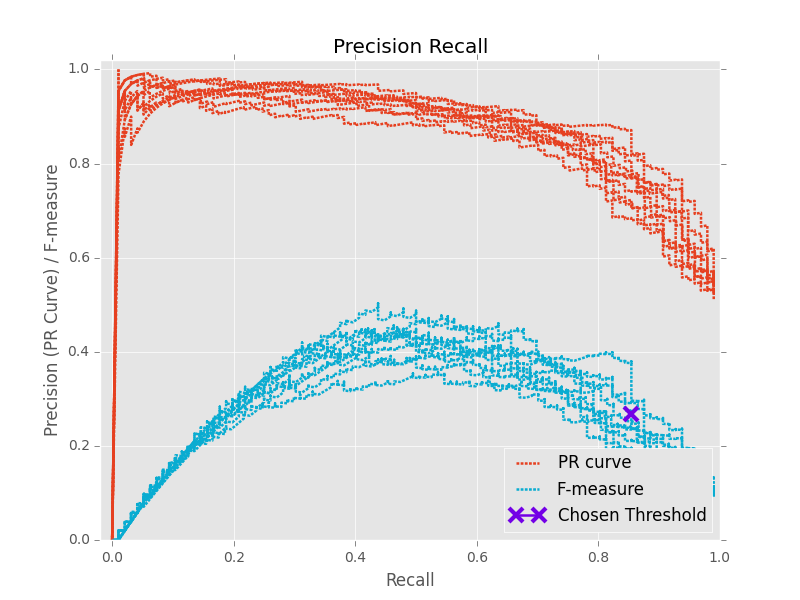
\includegraphics[width=\textwidth]{fig/LogReg_FindThreshold_PrCurve_coarse}
        \caption{Log Reg Pr Curves - Coarse}
    \end{subfigure}%
    ~
    \begin{subfigure}[t]{0.5\textwidth}
        \centering
        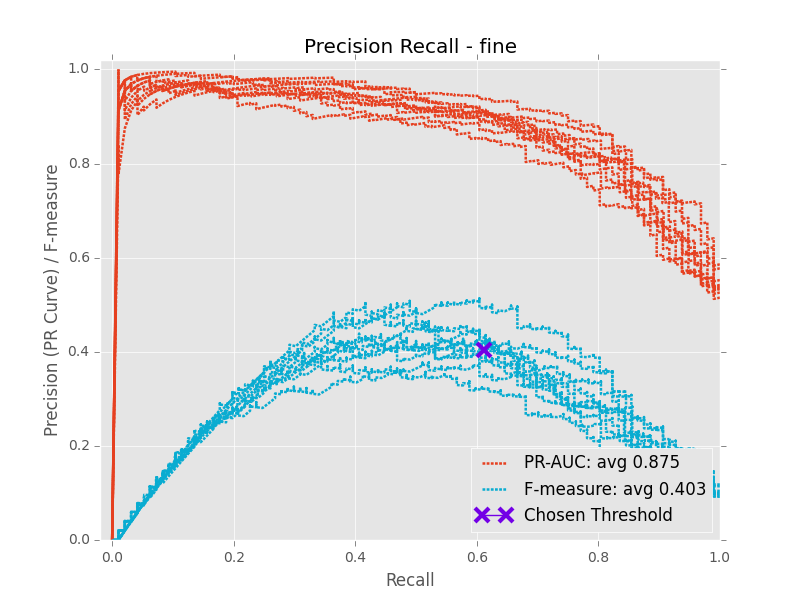
\includegraphics[width=\textwidth]{fig/LogReg_FindThreshold_PrCurve_fine}
        \caption{Log Reg Pr Curves - Fine}
    \end{subfigure}
    \caption{The Fine default threshold occurs at a point on the PR curve associated with a higher
    F-measure score compared to the Coarse curves.}
    \label{fig:LogRegThreshPr}
\end{figure*}
\FloatBarrier


\FloatBarrier
\begin{figure*}[!htb]
    \centering
    \begin{subfigure}[t]{0.5\textwidth}
        \centering
        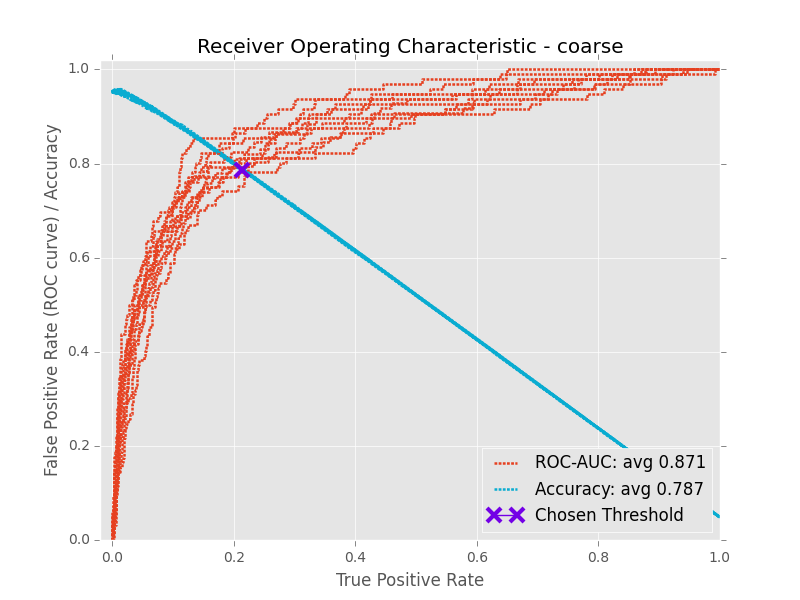
\includegraphics[width=\textwidth]{fig/LogReg_FindThreshold_RocCurve_coarse}
        \caption{Log Reg ROC Curves - coarse}
    \end{subfigure}%
    ~
    \begin{subfigure}[t]{0.5\textwidth}
        \centering
        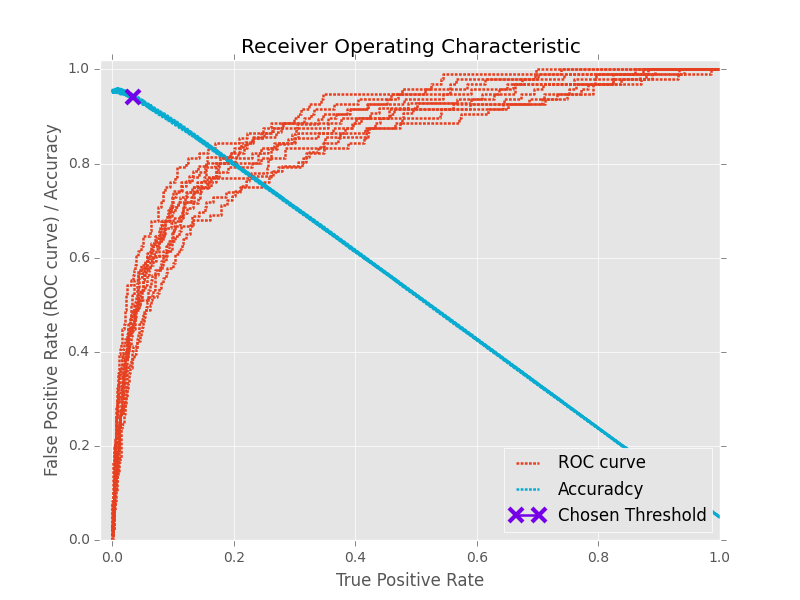
\includegraphics[width=\textwidth]{fig/LogReg_FindThreshold_RocCurve_fine}
        \caption{Log Reg ROC Curves - fine}
    \end{subfigure}
    \caption{Fine has a higher accuracy than coarse at the default threshold for the Logit classifier.}
    \label{fig:LogRegThreshAcc}
\end{figure*}
\FloatBarrier




\FloatBarrier
\begin{figure*}[!htb]
    \centering
    \begin{subfigure}[t]{0.5\textwidth}
        \centering
        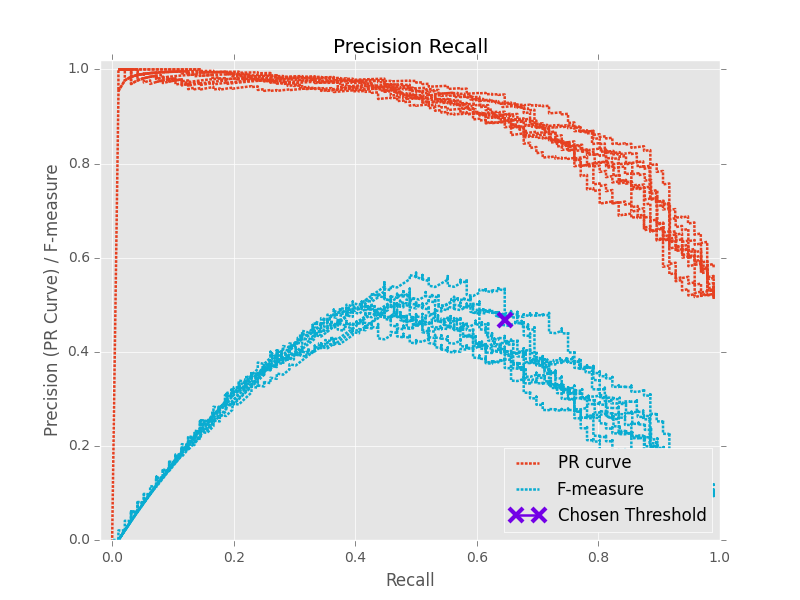
\includegraphics[width=\textwidth]{fig/SVM_FindThreshold_PrCurve_coarse}
        \caption{SVM Pr Curves - Coarse}
    \end{subfigure}%
    ~
    \begin{subfigure}[t]{0.5\textwidth}
        \centering
        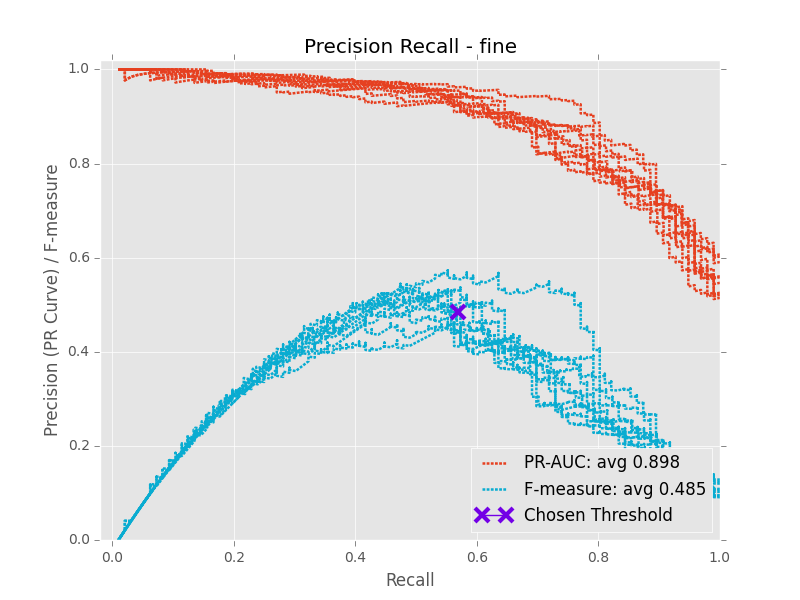
\includegraphics[width=\textwidth]{fig/SVM_FindThreshold_PrCurve_fine}
        \caption{SVM Pr Curves - Fine}
    \end{subfigure}
    \caption{SVM results for PR curves and F-measure have Coarse and Fine picking
    different parts of the curves for their respective thresholds. This results in a slight
    advantage for Fine at the default threshold, similar to the results for the Logit classifier.}
    \label{fig:SVMThreshPr}
\end{figure*}
\FloatBarrier


\FloatBarrier
\begin{figure*}[!htb]
    \centering
    \begin{subfigure}[t]{0.5\textwidth}
        \centering
        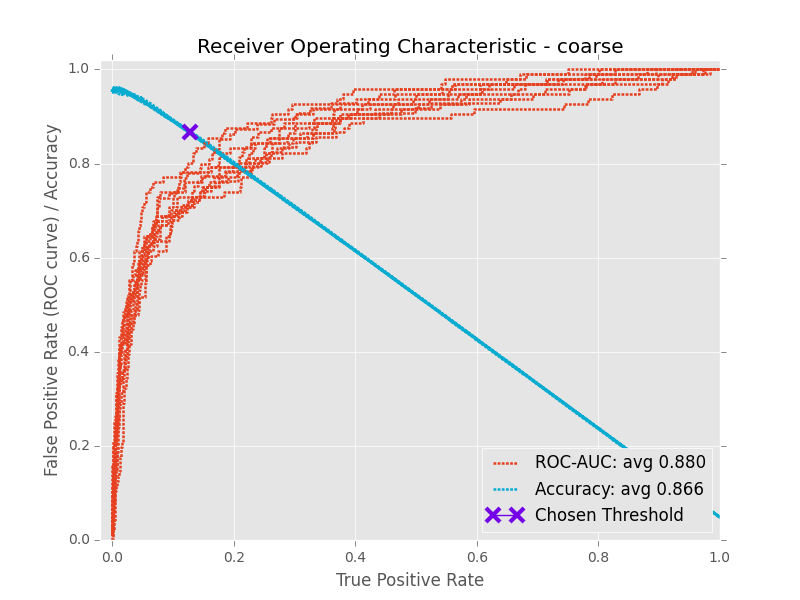
\includegraphics[width=\textwidth]{fig/SVM_FindThreshold_RocCurve_coarse}
        \caption{SVM ROC Curves - Coarse}
    \end{subfigure}%
    ~
    \begin{subfigure}[t]{0.5\textwidth}
        \centering
        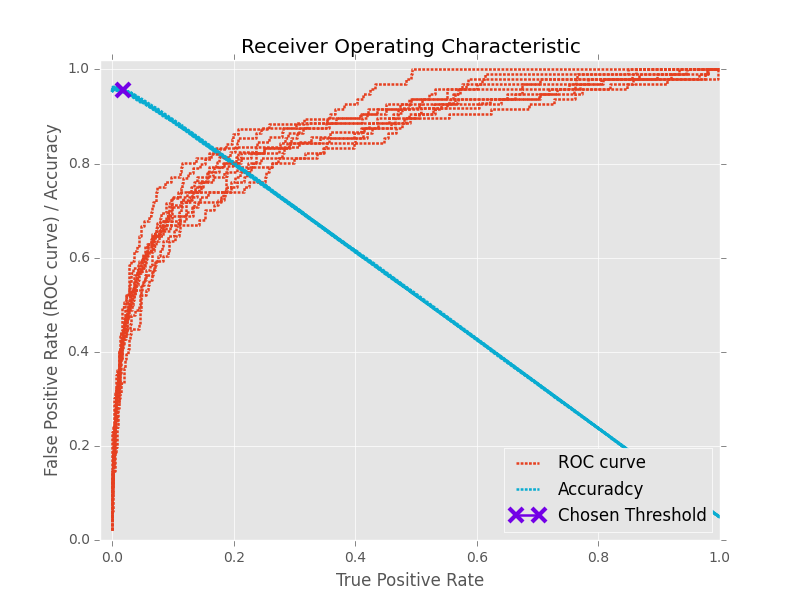
\includegraphics[width=\textwidth]{fig/SVM_FindThreshold_RocCurve_fine}
        \caption{SVM ROC Curves - Fine}
    \end{subfigure}
    \caption{SVM accuracy results are similar between Coarse and Fine.}
    \label{fig:SVMThreshRoc}
\end{figure*}
\FloatBarrier






\section{Active vs Passive curves}
\par The plots in \textit{Figures \ref{fig:runActPassLogReg_pr}-\ref{fig:rnd20LogRegRoc}}
were obtained with a round batch size of 100
and a starter set of 1040 instances out of the total 20098 instances.
The plots are the average of 10 folds, for each fold a test set of 2010 instances
is used. The test set remains constant throughout the rounds and contains a representative proportion
 of each of the classes. The starter set is chosen out of the remaining 18088 and it also contains representatives
 from each class in proportion to that class's prominence in the dataset. The 17048 non-test set, non-starter set
  instances are added to the training set in batches of 100. This results in total of 171 rounds, 170 batch selecting
  rounds and 1 starter set round. The Passive approach selects 100 random instances
   and adds them to the train set. The Active approach runs the classifier on the eligible instances, orders them
   by their uncertainty and adds the 100 most uncertain instances to the train set. Coarse and fine classifiers
   share the same starter set. During each round, Coarse and Fine classifiers are trained on their corresponding
 sets, which are independent of one another, metrics are outputted on the held out test set which is the same for
 both Coarse and Fine.


\FloatBarrier
\subsection{Plots for Logistic Regression Active vs Passive curves}
\begin{figure}[!htb]
	\centering
    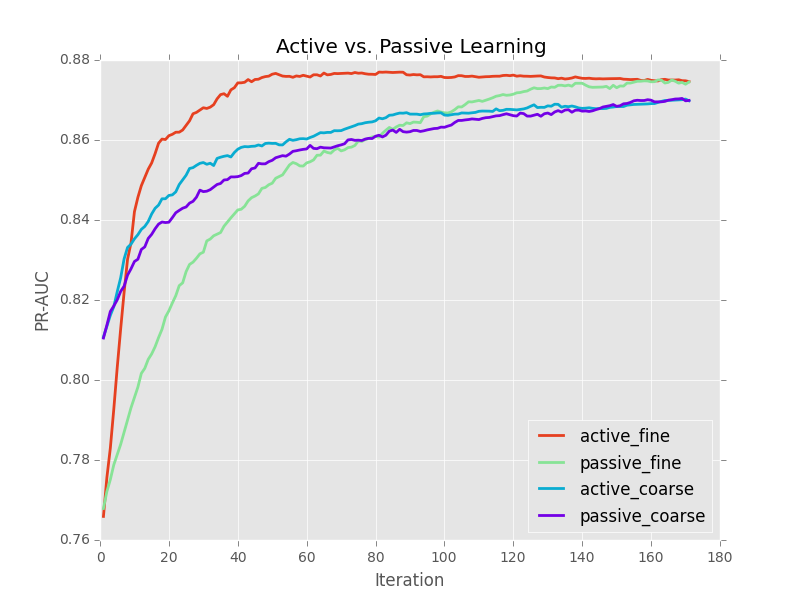
\includegraphics[width=1.0\columnwidth]{fig/runActPassLogReg_pr}
    \caption{The PR-AUC curves for rounds with the Logistic
Regression classifier conforms to expectations, with Active Fine having
the highest performance, and Active outperforming Passive for both Coarse
and Fine classifier types.}
\label{fig:runActPassLogReg_pr}
\end{figure}
\FloatBarrier

\FloatBarrier
\begin{figure}[!htb]
	\centering
    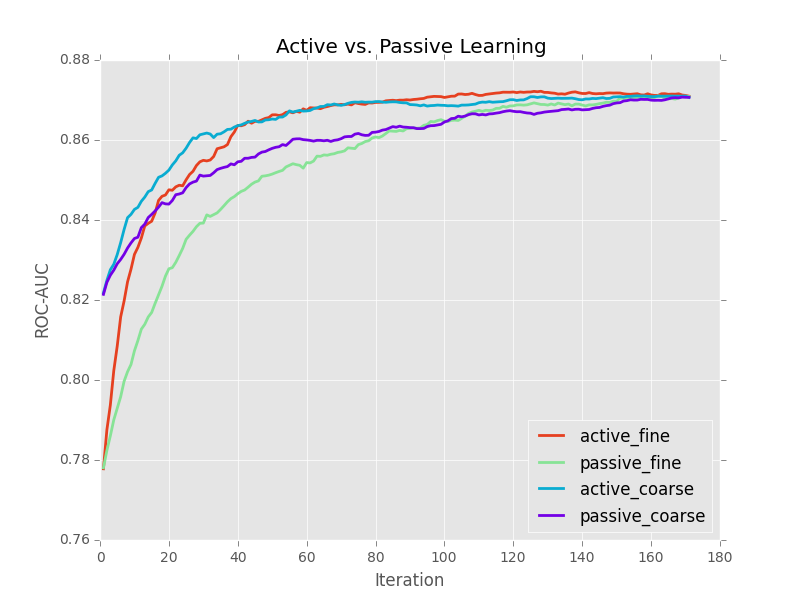
\includegraphics[width=1.0\columnwidth]{fig/runActPassLogReg_roc}
    \caption{The ROC-AUC curves for rounds with the
Logistic Regression classifier. The active curves beat out the passive
curves for both Coarse and Fine. Note that Active Fine ROC curve doesn't
converge to the Active Coarse ROC curve until round 40. This is contrasted
to a dominance of the Active Fine PR curve after round 10.}
\label{fig:runActPassLogReg_roc}
\end{figure}
\FloatBarrier


\FloatBarrier
\begin{figure*}[!htb]
    \centering
    \begin{subfigure}[t]{0.75\textwidth}
        \centering
        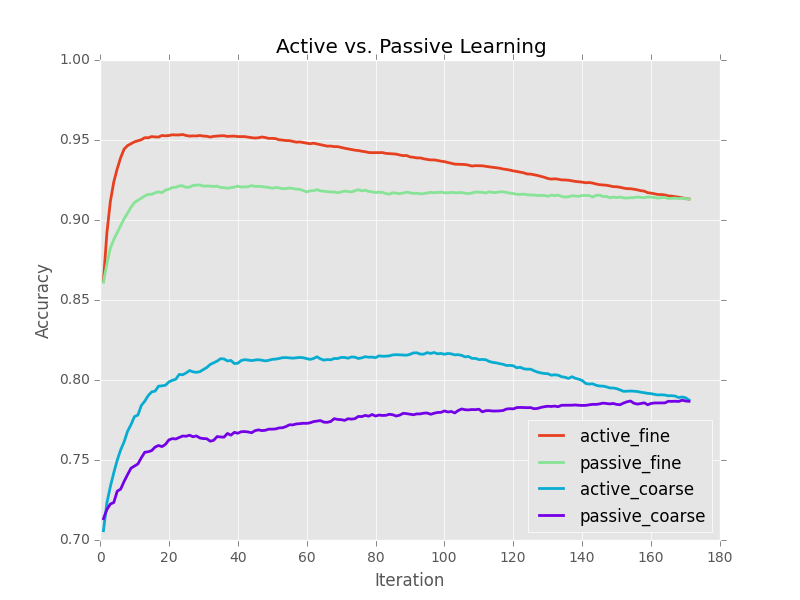
\includegraphics[width=\textwidth]{fig/runActPassLogReg_acc}
        \caption{Logit accuracy}
    \end{subfigure}% %~

    \begin{subfigure}[t]{0.75\textwidth}
        \centering
        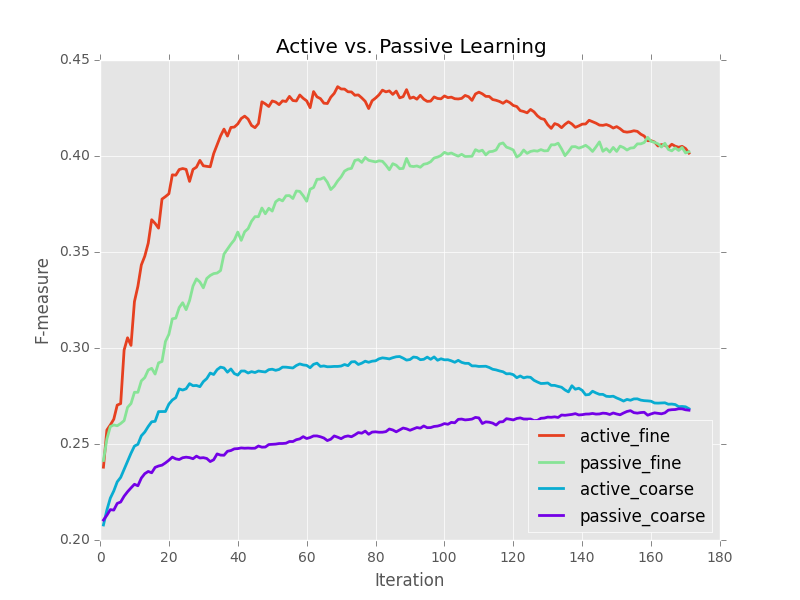
\includegraphics[width=\textwidth]{fig/runActPassLogReg_f1}
        \caption{Logit F-measure}
    \end{subfigure}
    \caption{The accuracy of the classifiers stays at
roughly the same rate throughout the rounds; this is due to an effective
weighting scheme. Both curves show a dominance of Fine over Coarse and
Active over Passive.}
    \label{fig:ActiveVsPassiveAccFmesLR}
\end{figure*}
\FloatBarrier


\par Note that the Active Fine PR-AUC curve
surpasses Active Coarse after round 10 while the Active Fine ROC-AUC curve is still well below the
 Active Coarse at that round. These curves are shown in \textit{Figures \ref{fig:rnd20LogRegPr}-
 \ref{fig:rnd20LogRegRoc}}. This is counter-intuitive, because according to a proof in Davis \cite{DavisRocPr}
 ``For a fixed number of positive and negative examples, one curve dominates a second curve in
 ROC space if and only if the first dominates the second in Precision-Recall space". The theorem uses the
 following definition of dominance: that every value in the first curve is above the corollary value in
 second curve. The correlation between PR and ROC curves is that Recall in the PR curve is equivalent to
 the True Positive Rate in the ROC curve. The average PR-AUC concept is different than that of a plot of
 PR curves for a round, but if all of the PR curves for Fine dominate the curves for Coarse then we would
  expect all of the ROC curves for Fine to dominate the ROC curves for coarse and both the ROC-AUC and PR-AUC
   averages for Fine to be greater than that for Coarse. However it is shown in \textit{Figure \ref{fig:rnd20LogRegPr}}
   that the PR curves for Fine do not completely dominate the PR curves for coarse, and similarly for the ROC curves
   in \textit{Figure \ref{fig:rnd20LogRegRoc}}. Active Fine PR-AUC curve does not satisfy the theorem's
   definition of dominance, since each individual ROC and PR curve contains intersection points between
   Coarse and Fine. Thus given that the average PR-AUC for Fine is great at round 20 than average Coarse PR-AUC,
   this relationship is not expected to hold between the average ROC-AUC curves.
   \par According to Davis \cite{DavisRocPr}, a large change in the number of false positives can still yield
   only a small change in the number of false positives and thus not affect ROC curve performance. However,
   Davis states, ``Precision, on the other hand, by comparing false positives to true positives rather than true
   negatives, captures the effect of the large number (incorrectly classified) of negative examples on the
   algorithm's performance" \cite{DavisRocPr}. Since our dataset demonstrates a heavy class imbalance with
    a roughly 1:20 ratio of Positive to Negative instances, the algorithm's ability to classify negative instances
    should be taken into account when considering overall classifier performance. The PR curve's ability to capture
    and have a greater sensitivity to the increased number of False Positives, reveals the advantage that the Fine
    classifier has over the Coarse classifier. This justifies purchasing Fine grained labels over Coarse grained labels
    to improve classifier performance.

\FloatBarrier
\begin{figure*}[!htb]
    \centering
    \begin{subfigure}[t]{0.5\textwidth}
        \centering
        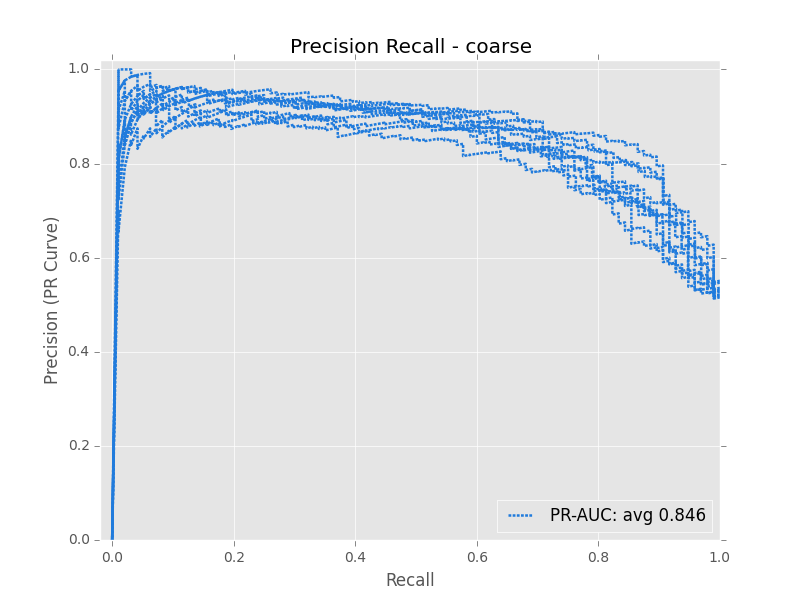
\includegraphics[width=\textwidth]{fig/RndNum_20_LogReg_PrCurves_coarse}
        \caption{Coarse PR curves at Round 20}
    \end{subfigure}%
    ~
    \begin{subfigure}[t]{0.5\textwidth}
        \centering
        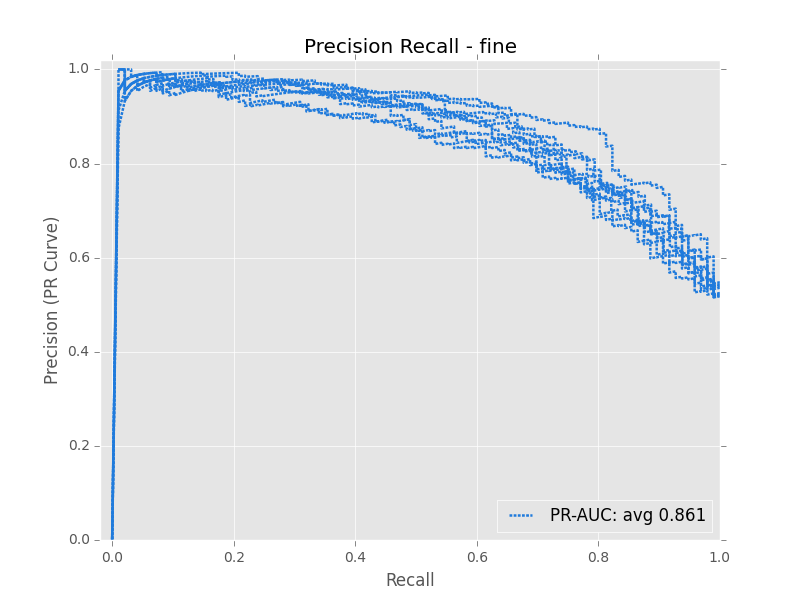
\includegraphics[width=\textwidth]{fig/RndNum_20_LogReg_PrCurves_fine}
        \caption{Fine PR curves at Round 20}
    \end{subfigure}
    \caption{PR curves for each fold at Round 20}
    \label{fig:rnd20LogRegPr}
\end{figure*}
\FloatBarrier



\FloatBarrier
\begin{figure*}[!htb]
    \centering
    \begin{subfigure}[t]{0.5\textwidth}
        \centering
        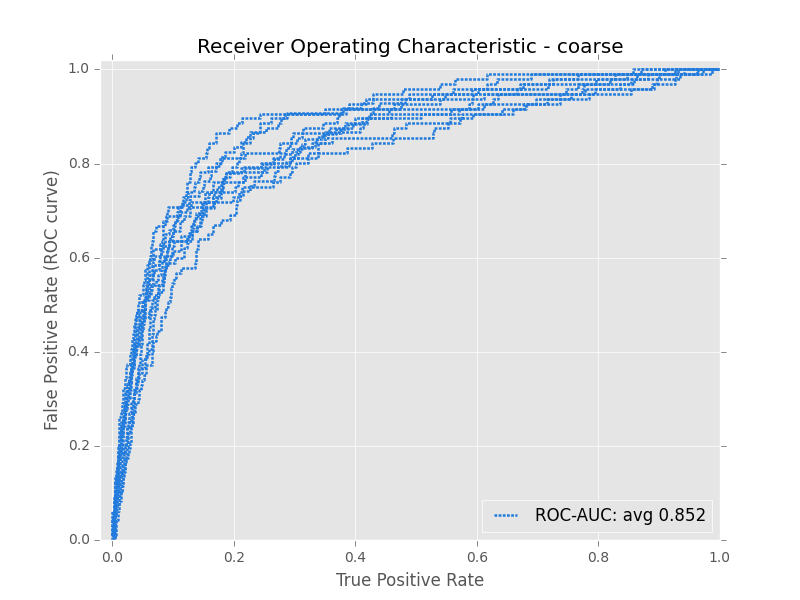
\includegraphics[width=\textwidth]{fig/RndNum_20_LogReg_RocCurves_coarse}
        \caption{Coarse ROC curves at Round 20}
    \end{subfigure}%
    ~
    \begin{subfigure}[t]{0.5\textwidth}
        \centering
        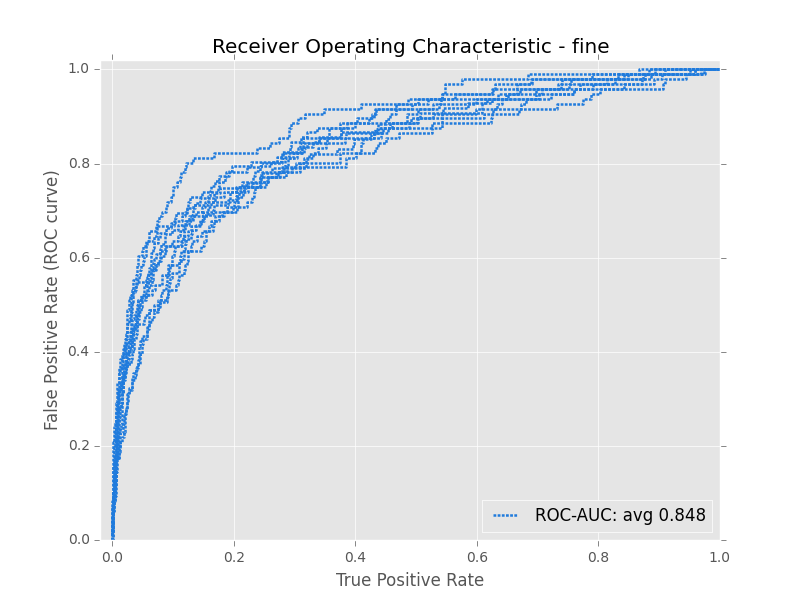
\includegraphics[width=\textwidth]{fig/RndNum_20_LogReg_RocCurves_fine}
        \caption{Fine ROC curves at Round 20}
    \end{subfigure}
    \caption{ROC curves for each fold at Round 20}
    \label{fig:rnd20LogRegRoc}
\end{figure*}
\FloatBarrier








\clearpage

\subsection{Plots for SVM Active vs Passive curves}
\par The SVM Active vs Passive experiment is performed with the same methodology
as the previous section detailed with the exception that a SVM classifier is
substituted for the Logit classifier. Due to the greater advantage of average
PR-AUC in the Logit classifier, the SVM is not used in the Fixed Fine ratio
experiments in section \ref{ffrSection} Plots for Fine Fixed Ratio experiments.

\FloatBarrier
\begin{figure}[!htb]
	\centering
    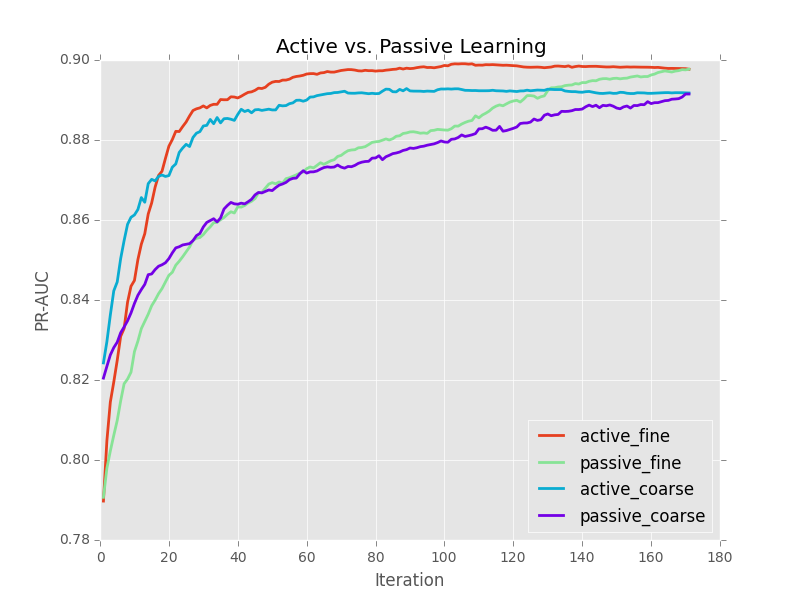
\includegraphics[width=1.0\columnwidth]{fig/runActPassSVM_pr}
    \label{fig:ActiveVsPassivePRSVM}
    \caption{The PR AUC curves for SVM show a slight advantage for Active Fine,
     similar to the Logit results.}
\end{figure}
\FloatBarrier

\FloatBarrier
\begin{figure}[!htb]
	\centering
    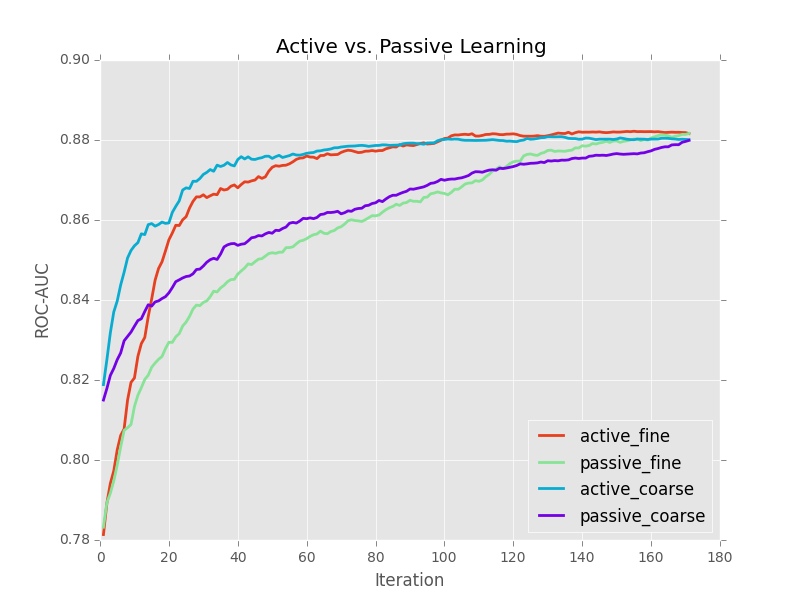
\includegraphics[width=1.0\columnwidth]{fig/runActPassSVM_roc}
    \label{fig:ActiveVsPassiveROCSVM}
    \caption{The ROC AUC curves for SVM match the Logit results, the convergence of
     Active Fine to Active Coarse takes slightly longer, round 60 compared to round 40.}
\end{figure}
\FloatBarrier


%\FloatBarrier
%\begin{figure}[!htb]
%	\centering
%    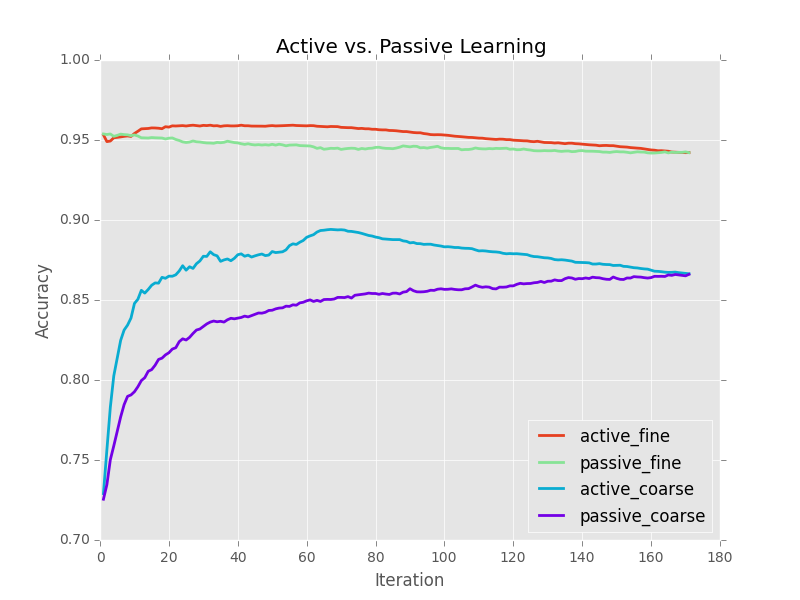
\includegraphics[width=1.0\columnwidth]{fig/runActPassSVM_acc}
%    \label{fig:ActiveVsPassiveAccSVM}
%    \caption{accuracy is ok.}
%\end{figure}
%\FloatBarrier
%
%\FloatBarrier
%\begin{figure}[!htb]
%	\centering
%    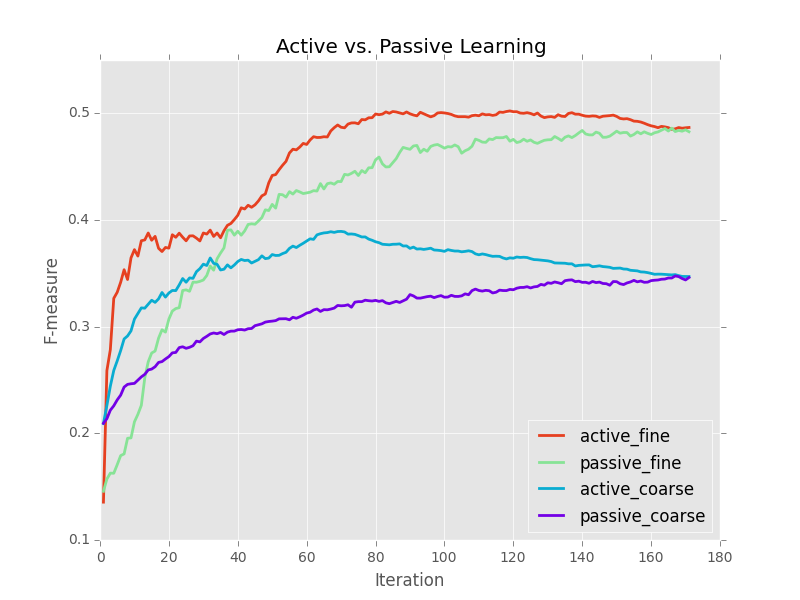
\includegraphics[width=1.0\columnwidth]{fig/runActPassSVM_f1}
%    \label{fig:ActiveVsPassiveF1SVM}
%    \caption{The active fine fmeasure has weird bump in it}
%\end{figure}
%\FloatBarrier


\clearpage

\section{Plots for Fine Fixed Ratio experiments}
\label{ffrSection}
\par The strategy is changed from purchasing a set number of instances
    per round to having a set budget per round and spending a portion of that budget
    on fine and coarse grained labels. The Fine Fixed Ratio (FFR), ranges from 0.0 to
    1.0 in increments of 0.1. Note that the FFR 0.0 should roughly correlate to the
    Active Coarse curve shown in \textit{Figure \ref{fig:runActPassLogReg_pr}}. Likewise
    the Active Fine curve should roughly correlate to the FFR 1.0 curve. However, the correlation
    is not exact since the FFR experiments use a combination classifier, it trains Fine and
    Coarse classifiers on a starter set of the same size and proportion as used in the
    Logit Active vs Passive experiment, then uses the confidence of both of those classifiers and
    the end prediction is the max of the two classifiers. Thus even for the FFR 0.0 and FFR 1.0
    the starter set trained Fine or Coarse classifier still contributes to the PR-AUC curve
    even at the final round 180. The results are an average of 10 folds.

    \par To determine the number of instances to purchase each round the FFR is multiplied by the
    round budget of 100, then the round budget for the coarse labels are purchased at a cost of 1.0.
    The cost of the fine labels will vary and if a decimal occurs it is resolved by randomly purchasing
    an extra fine label with the probability of the decimal value. For example, if the fine cost is 16 and
    FFR is 0.5, 50 instances are bought for coarse and 3.125 instances are
    bought for fine. The remainder 0.125 is then turned into a 0.125 chance for any round to
    purchase an extra fine label. The round size for the FFR 1.0 curve is very small, with only
    7 labels purchased per iteration.

\FloatBarrier
\begin{figure}[!htb]
	\centering
    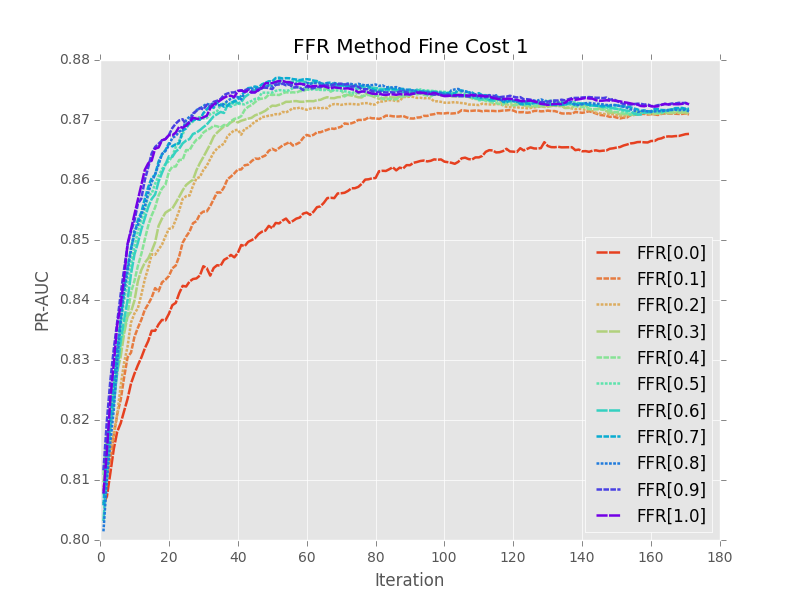
\includegraphics[width=1.0\columnwidth]{fig/ParamsFFR_PR_Cost1_rnds0_180}
    \label{fig:ParamsFFR_PR_Cost1_rnds0_180}
    \caption{For this curve the fine and coarse grain labels
    both have a cost of 1. The purple 1.0 curve shows that if only fine-grained labels
    are purchased, the highest performing PR-AUC can be obtained. All FFR ratios end at the same round
    since the cost of the Fine and Coarse instances is the same the budget}
\end{figure}
\FloatBarrier


\FloatBarrier
\begin{figure}[!htb]
	\centering
    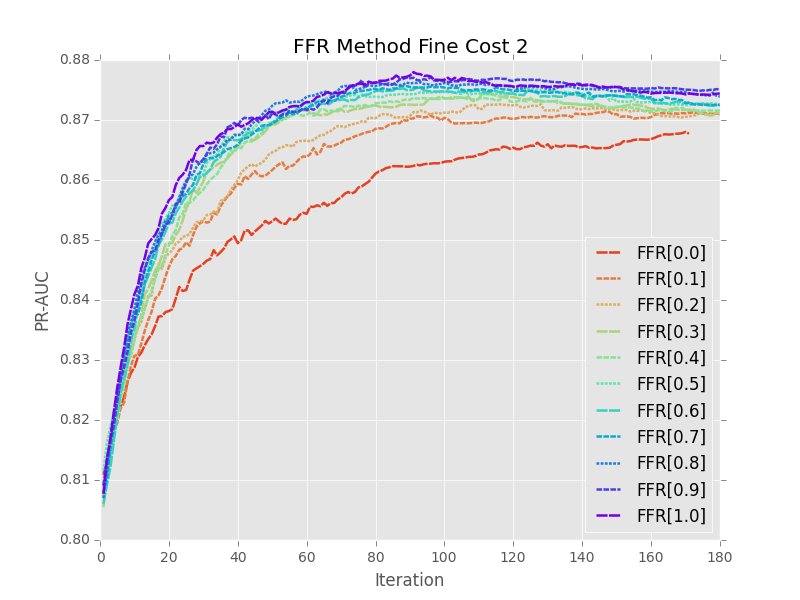
\includegraphics[width=1.0\columnwidth]{fig/ParamsFFR_PR_Cost2_rnds0_180}
    \label{fig:ParamsFFR_PR_Cost2_rnds0_180}
    \caption{At fine cost 2, advantage of the higher FFR values decreases but the ordering
    of the curves remains unchanged.}
\end{figure}
\FloatBarrier



\FloatBarrier
\begin{figure}[!htb]
	\centering
    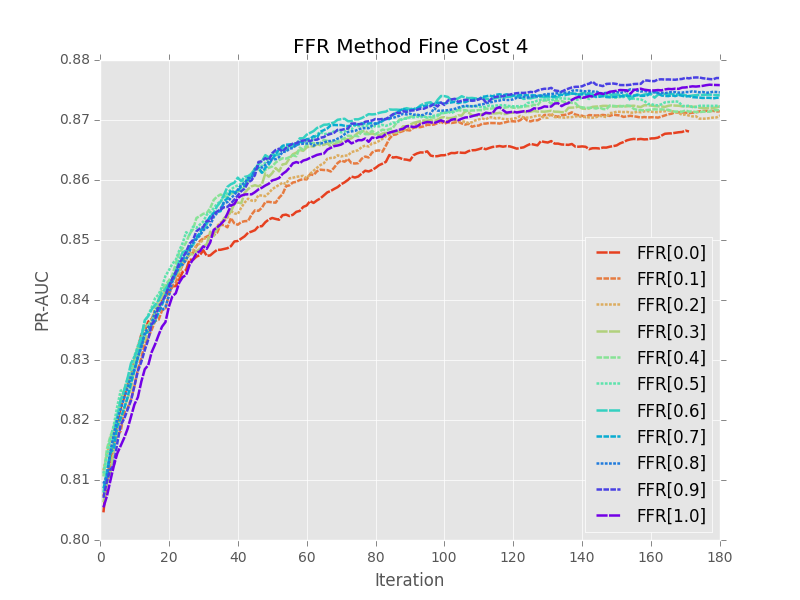
\includegraphics[width=1.0\columnwidth]{fig/ParamsFFR_PR_Cost4_rnds0_180}
    \label{fig:ParamsFFR_PR_Cost4_rnds0_180}
    \caption{At fine cost 4, the highest FFR 1.0 is no longer preferred, the
    cost is to high for Fine instances PR-AUC utility to overcome the PR-AUC
    increase gained by purchasing more Coarse instances.}
\end{figure}
\FloatBarrier


\FloatBarrier
\begin{figure}[!htb]
	\centering
    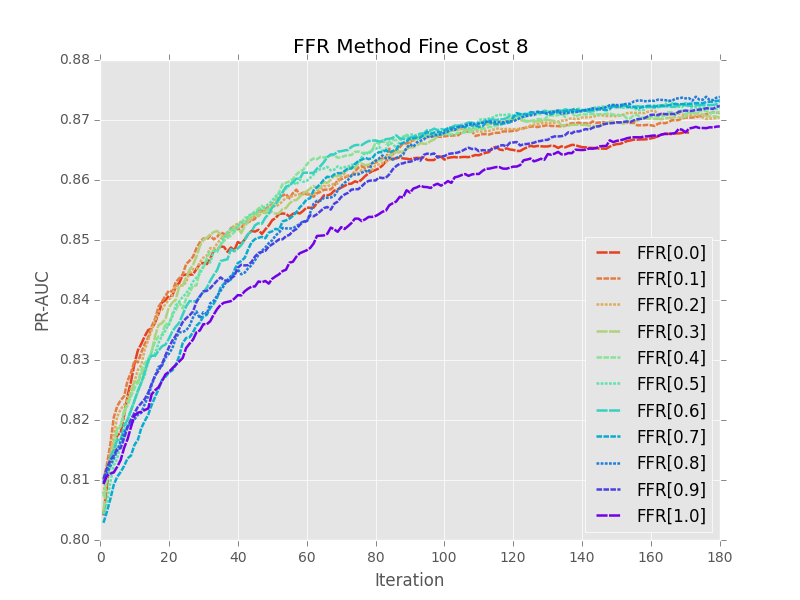
\includegraphics[width=1.0\columnwidth]{fig/ParamsFFR_PR_Cost8_rnds0_180}
    \label{fig:ParamsFFR_PR_Cost8_rnds0_180}
    \caption{At fine cost 8 the middle FFR values outperform the extreme values
    for rounds 0 to 180.}
\end{figure}
\FloatBarrier

\FloatBarrier
\begin{figure}[!htb]
	\centering
    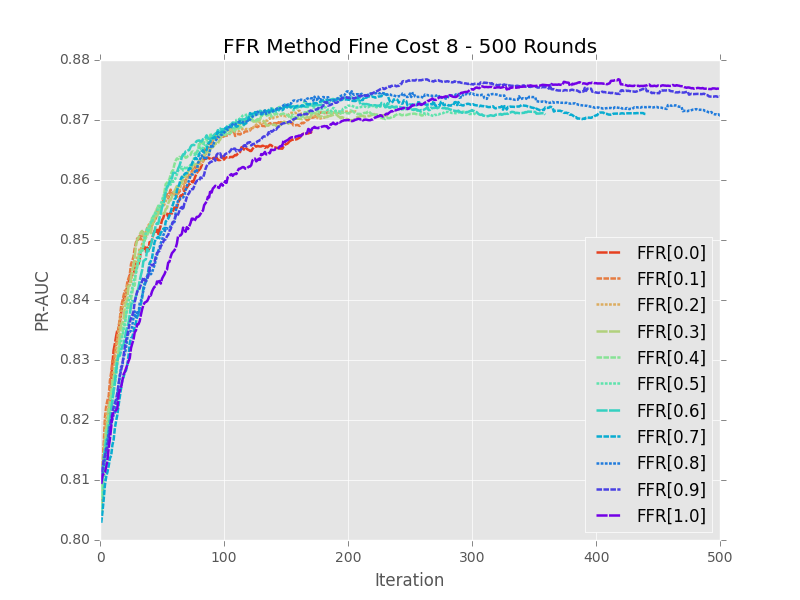
\includegraphics[width=1.0\columnwidth]{fig/ParamsFFR_PR_Cost8_rnds0_500}
    \label{fig:ParamsFFR_PR_Cost8_rnds0_500}
    \caption{This shows the iterations continuing through round 500, the curves
    with the higher fine rates eventually settle to the same end point that the
    curves with the high rates of coarse labels purchased achieved at previous
    iterations.}
\end{figure}
\FloatBarrier

\FloatBarrier
\begin{figure}[!htb]
	\centering
    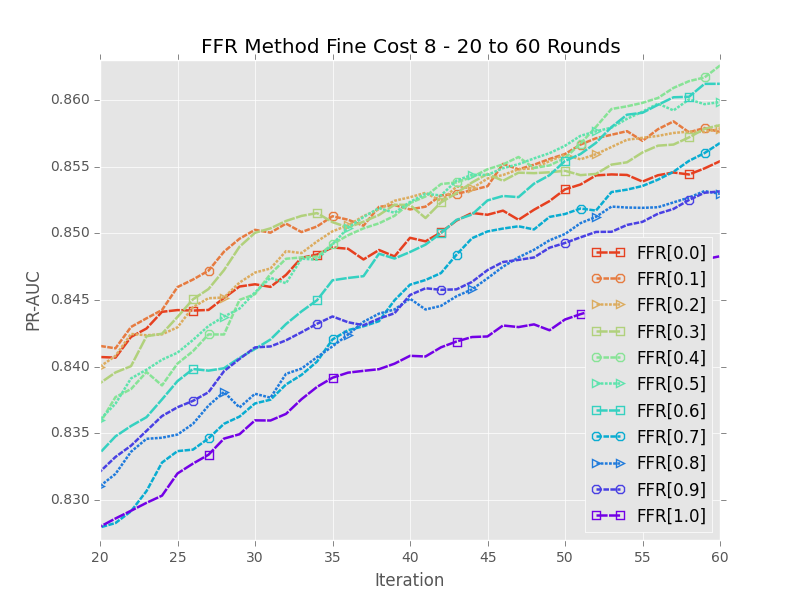
\includegraphics[width=1.0\columnwidth]{fig/ParamsFFR_PR_Cost8_rnds20_60}
    \label{fig:ParamsFFR_PR_Cost8_rnds20_60}
    \caption{The fine cost 8 curves shown expanding the rounds 20-60. If a round budget of 40
    occurs than the recommended Fine Fixed Ratio would be 0.2}
\end{figure}
\FloatBarrier


\FloatBarrier
\begin{figure}[!htb]
	\centering
    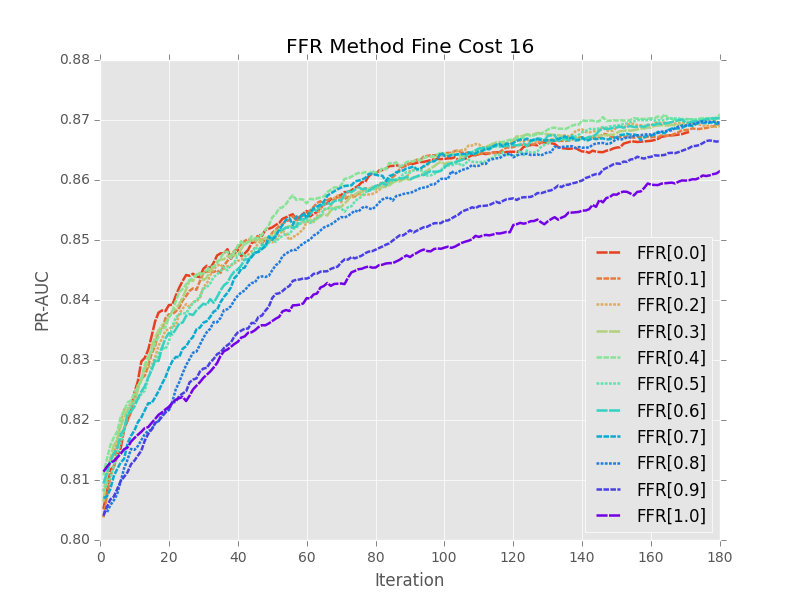
\includegraphics[width=1.0\columnwidth]{fig/ParamsFFR_PR_Cost16_rnds0_180}
    \label{fig:ParamsFFR_PR_Cost16_rnds0_180}
    \caption{The fine cost is increased to 16. The cost is to high for the fine label advantage to offset
    the decreased number of instances purchased.}
\end{figure}
\FloatBarrier

%
%\FloatBarrier
%\begin{figure}[!htb]
%	\centering
%    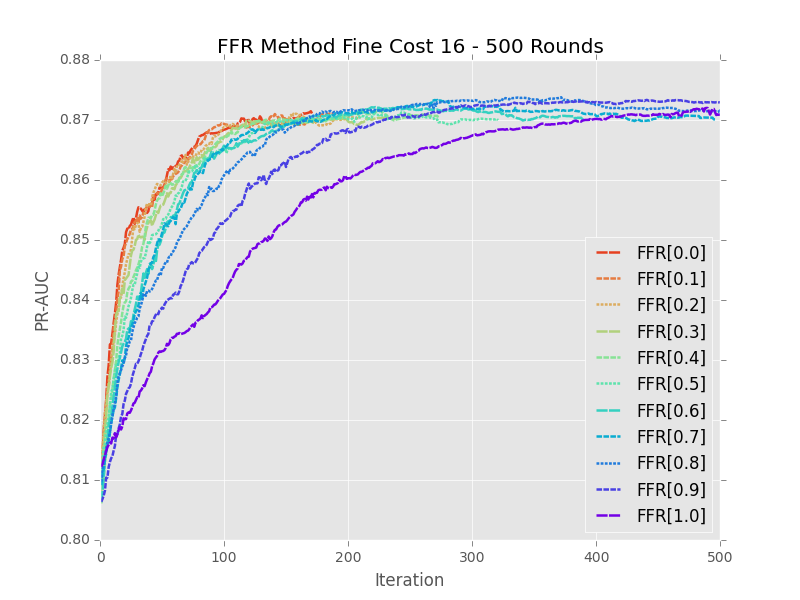
\includegraphics[width=1.0\columnwidth]{fig/FFR_PR_Cost16_rnds0_500}
%    \label{fig:FFR_PR_Cost16_rnds0_500}
%    \caption{This shows the iterations continuing through round 500, the curves
%    with the higher fine rates eventually settle to the same end point that the
%    curves with the high rates of coarse labels purchased achieved at previous
%    iterations.}
%\end{figure}
%\FloatBarrier


%
%
%\FloatBarrier
%\begin{figure}[!htb]
%	\centering
%    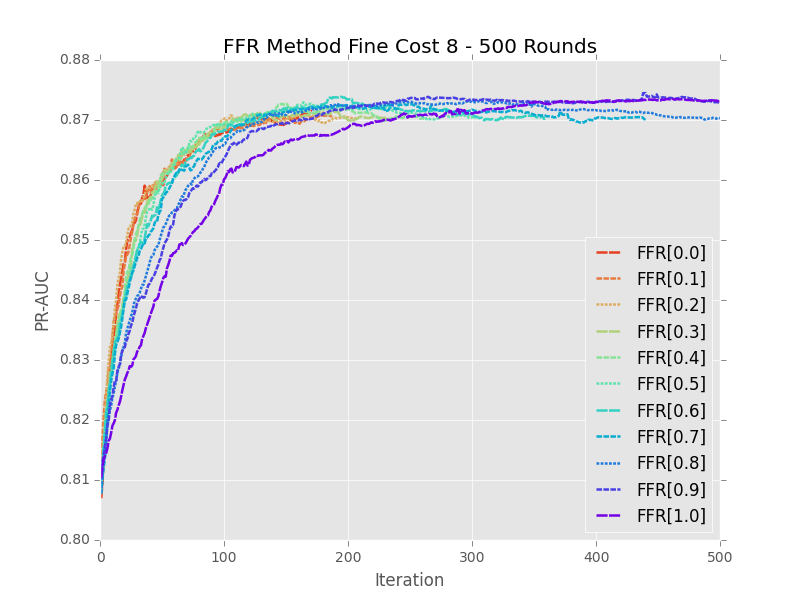
\includegraphics[width=1.0\columnwidth]{fig/FFR_PR_Cost8_rnds0_500}
%    \label{fig:FFR_PR_Cost8_rnds0_500}
%    \caption{The extended picture of the FFR cost 8. The round size for FFR 1.0
%    is small, only 13 instances purchase per iteration.}
%\end{figure}
%\FloatBarrier


%
%\FloatBarrier
%\begin{figure}[!htb]
%	\centering
%    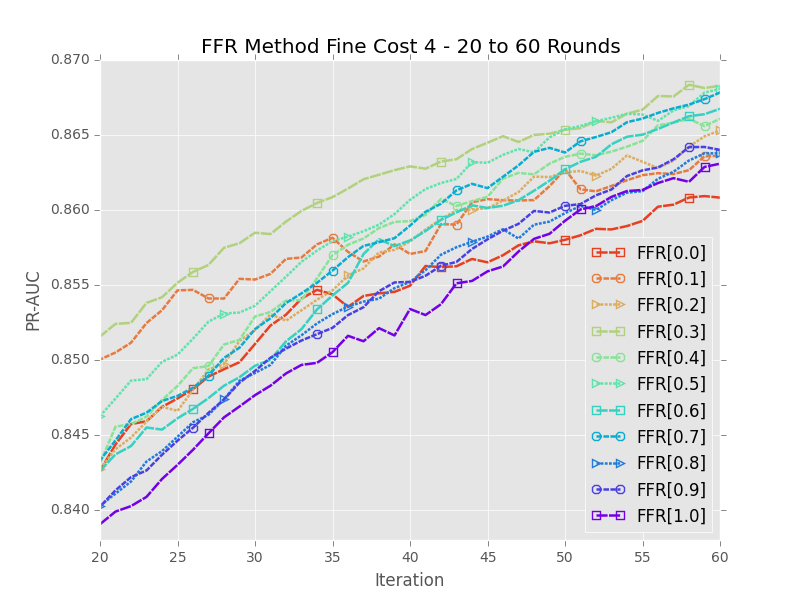
\includegraphics[width=1.0\columnwidth]{fig/FFR_PR_Cost4_rnds20_60}
%    \label{fig:FFR_PR_Cost4_rnds20_60}
%    \caption{The fine cost 4 curves shown expanding the rounds 20-60.}
%\end{figure}
%\FloatBarrier


%\FloatBarrier
%\begin{figure}[!htb]
%	\centering
%    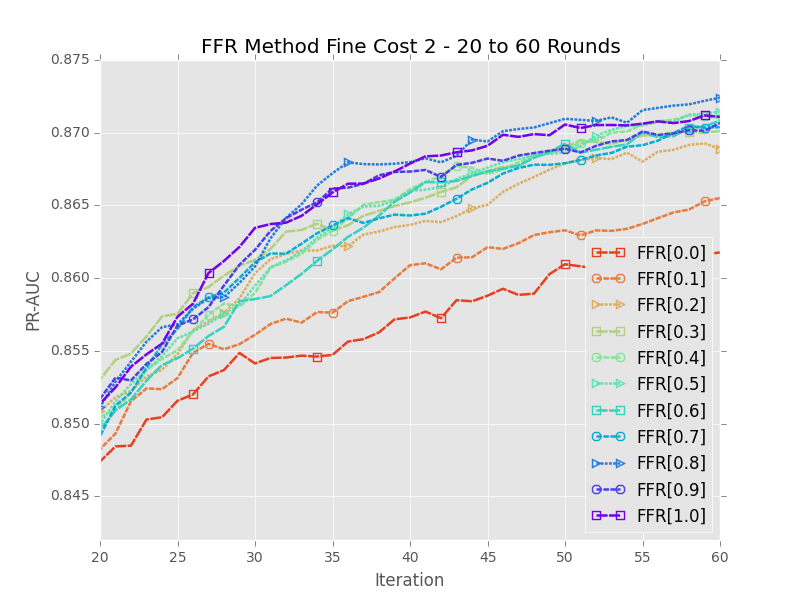
\includegraphics[width=1.0\columnwidth]{fig/FFR_PR_Cost2_rnds20_60}
%    \label{fig:FFR_PR_Cost2_rnds20_60}
%    \caption{The fine cost 2 curves shown expanding rounds 20-60.}
%\end{figure}
%\FloatBarrier



\chapter{Conclusions and Future Work}
\par I should probably do the Bandit experiments.










%% backmatter is needed at the end of the main body of your thesis to
%% set up page numbering correctly for the remainder of the thesis
\backmatter

%% Start the correct formatting for the appendices
%\appendix
%
%\chapter{Tuning the fine grained classes}
%\par All the data and results for tuning the fine grained classes.

%% Bibliography goes here (You better have one)
%% BibTeX is your friend
%\bibliographystyle{plain}
\bibliographystyle{IEEEtran}
\bibliography{IEEEabrv,nuthesis}
%% Pull in all the entries in the bibtex file. Is is a useful trick to
%% check all your references.
\nocite{*}


%% Index go here (if you have one)

\end{document}
\endinput
%%
%% End of file `thesis-test.tex'.
